\documentclass[
        oneside,      %%coloque  % no in\'icio desta linha para imprimir frente e verso 
        english,			
%	french,				
%	spanish, 
        brazil			 
        ]{abntbibufjf}


\usepackage[T1]{fontenc}		
\usepackage[utf8]{inputenc}		%% Para converter automaticamente acentos como digitados normalmente no teclado. Mude utf8 para latin1 se precisar. 

\usepackage{lmodern} %no caso do modelo Latex, pode-se usar a fam\'ilia de fontes lmodern como aqui indicado, no lugar de Arial e Times New Roman.

\usepackage{amsmath, xparse}
\usepackage{lastpage}			
\usepackage{indentfirst}		
\usepackage{color}			
\usepackage{graphicx}			
\usepackage{microtype} 
\usepackage{hyperref}
\usepackage{xurl}
\usepackage{float}
\usepackage{subcaption}
\usepackage{pdfpages}
%\usepackage{bmatrix}
%% -----------------------------------------------------------------------------

%% Obs.: Alguns acentos foram omitidos.

\titulo{T\'itulo} %% Colocar, dentro de chaves {}, o t\'itulo do trabalho. 
\subtitulo{subt\'itulo}  %% Colocar % no in\'icio desta linha se nao tiver subt\'itulo 
\autor{Guilherme Sebastião Pinhero Lopes} %%Colocar, dentro de chaves {}, o nome completo do autor
\autorVirg{Sobrenome, Nome do autor} %%Colocar o sobrenome do autor, separado por v\'rgula, antes do restante do nome do autor. Ex.: Santos, Maria dos
\local{Juiz de Fora} %%Governador Valadares % N\~ao usar MG.
\data{Ano} %%Colocar o ano da entrega. Por exemplo, 2019. N\~ao usar m\^es.
\orientador[Orientador:]{Nome e sobrenome} %%Se precisar, troque [Orientador:] por [Orientadora:]
\coorientador[Coorientador:]{Nome e sobrenome} %% Colocar ``%'' no in\'icio desta linha se n\~ao tiver coorientador. Se precisar, troque por [Cooorientadora:]. 
\orientadorTitulo{Titula\c{c}\~ao} %%Colocar, dentro de chaves {}, a titula\c{c}\~ao do(a) orientador(a). Por exemplo, Prof. Dr.
\coorientadorTitulo{Titula\c{c}\~ao} %%Colocar, dentro de chaves {}, a titula\c{c}\~ao do(a) cooorientador(a). 
\instituicao{Universidade Federal de Juiz de Fora}
\faculdade{Faculdade de Engenharia} %%Colocar, dentro de chaves {}, o nome da faculdade ou do instituto.
\programa{PROGRAMA DE PÓS GRADUAÇÃO EM ENGENHARIA ELÉTRICA} %%Colocar, dentro de chaves {}, o nome do curso. Por exemplo: Programa de P\'os\mbox{-Gra}dua\c{c}\~ao em Matem\'atica
\objeto{Disserta\c{c}\~ao (Mestrado)}  %%Tese (Doutorado)  %%%Trabalho de Conclus\~ao de Curso (gradua\c{c}\~ao)
\natureza{Disserta\c{c}\~ao  %%Tese 
apresentada ao \insereprograma ~da   %% %%%Trabalho de conclus\~ao de curso apresentado \'a \inserefaculdade da %%%%SUBSTITUIR \'a POR ao SE FOR INSTITUTO    
Universidade Federal de Juiz de Fora como requisito parcial \`a obten\c{c}\~ao do 
t\'itulo de Mestre em  %%Doutor em    %%%grau de bacharel em 
Matem\'atica. %%Trocar Matem\'atica por outro, se precisar.
\'Area de concentra\c{c}\~ao: %%PREENCHER   %%%N\~ao usar esta linha se for trabalho de conclus\~ao de curso da gradua\c{c}\~ao
}

%% Abaixo, prencher com os dados da parte final da ficha catalografica
\finalcatalog{1. Palavra-chave. 2. Palavra-chave. 3. Palavra-chave. I. Sobrenome, Nome do orientador, orient. II. T\'itulo.} %% Aqui fica 
% escrito a palavra ``T\'itulo'' mesmo, nao o do trabalho. Se tiver coorientador, os dados ficam depois dos dados 
%% do orientador (II. Sobrenome, Nome do coorientador, coorient.) e antes de ``II. T\'itulo'', o qual passa a ``III. T\'itulo''.


\usepackage[round, numbers]{natbib} %para refer\^encias bibliogr\'aficas no sistema num\'erico com () na chamada da citacao. 

%Se for usar o sistema autor-data, colocar % antes de \usepackage acima e retirar % antes de \usepackage abaixo.

%\usepackage{natbib} %para o sistema autor-data

\begin{document}

%% ELEMENTOS PR\'E-TEXTUAIS


%% Capa. N\~ao entra na contagem da pagina\c{c}\~ao.
\inserecapa

%% Folha de rosto
\inserefolhaderosto

%% Ficha catalogr\'afica. AO IMPRIMIR, DEIXAR NO VERSO DA FOLHA DE ROSTO.
\inserecatalog  


%% Folha de aprovacao. Incluir mesmo que sem assinaturas. Assinaturas eletr\^onicas via SEI.
\begin{folhadeaprovacao}
\inicfolhaaprov
        
Aprovada em (dia) de (m\^es) de (ano) %%Preencher com a data 
   
\vfill
\begin{center} BANCA EXAMINADORA \end{center}
\assinatura{Ph.D. Rafael Antunes Nóbrega\ - Orientador \\ Universidade Federal de Juiz de Fora}  %%Orientadora
\assinatura{Ph.D. Igor Abritta Costa\ - Coorientador \\ Universidade Federal de Juiz de Fora}
\assinatura{Titula\c{c}\~ao Nome e sobrenome \\ Universidade ???}
\assinatura{Titula\c{c}\~ao Nome e sobrenome  \\ Universidade ??} 
%\assinatura{...} %%RETIRE O % E PREENCHA SE PRECISAR
%  \assinatura{...}
%  \assinatura{...}
\end{folhadeaprovacao}
\cleardoublepage 


%% Dedicatoria. OPCIONAL. N\~ao deve haver t\'itulo. Colocar ``%'' no in\'icio de cada das 3 linhas abaixo, caso n\~ao queira. 
 \begin{dedicatoria} 
  Dedico este trabalho ... 
 \end{dedicatoria}

 
%% Agradecimentos. OPCIONAL. Caso seja bolsista, inserir os devidos agradecimentos.
\begin{agradecimentos}
Agrade\c{c}o aos ... 
\end{agradecimentos}


%% Ep\'igrafe. OPCIONAL. Com os dados do autor. A obra usada na ep\'igrafe deve constar nas refer\^encias. 

% Quando at\'e 3 linhas: \'e obrigat\'orio o uso de aspas duplas.

%\begin{epigrafemenos} %%Ep\'igrafe com 3 ou menos linhas
%``Mas para que o produto de uma pesquisa científica possa ser publicado não basta que ele apresente um conteúdo de qualidade, também é exigida qualidade de forma.'' (MAR\c{C}AL JUNIOR, 2013, p. 19-20).
%\end{epigrafemenos}

%%Quando com mais de 3 linhas. 

\begin{epigrafemais} %%Ep\'igrafe com mais de 3 linhas 
	Elemento opcional, em que o autor apresenta uma cita\c{c}\~ao, seguida de indica\c{c}\~ao de autoria, relacionada com a                       
  mat\'eria tratada no corpo do trabalho. (ASSOCIA\c{C}\~AO BRASILEIRA DE NORMAS T\'ECNICAS, 2011, p. 2).
\end{epigrafemais}


%% RESUMOS

%% Resumo em Portugu\^es. OBRIGAT\'ORIO. \'E obrigat\'orio o uso de par\'agrafo \'unico.
\begin{resumo}

De acordo com a Associa\c{c}\~ao Brasileira de Normas T\'ecnicas NBR 6028 (2003, p.2), ``o resumo deve ressaltar 
o objetivo, o m\'etodo, os resultados e as conclus\~oes do documento. [...] Deve ser composto de uma sequ\^encia de frases 
concisas, afirmativas e n\~ao de enumera\c{c}\~ao de t\'opicos. Recomenda-se o uso de par\'agrafo \'unico.'' 
O resumo deve ter de 150 a 500 palavras. \\[18pt]
Palavras-chave: Palavra-chave. Palavra-chave. %Finalizadas por ponto e inicializadas por letra maiuscula.
\end{resumo}
 
 
%% Resumo em Ingl\^es. \'E obrigat\'orio o uso de par\'agrafo \'unico.
\begin{resumo}[ABSTRACT]
 \begin{otherlanguage*}{english}

Trata-se da vers\~ao do resumo em l\'ingua estrangeira para divulga\c{c}\~ao internacional. Segue as mesmas caracter\'isticas do resumo em 
l\'ingua vern\'acula. O t\'itulo \'e atribu\'ido de acordo com o idioma escolhido (ABSTRACT, em ingl\^es; RESUMEN, em espanhol; etc.), bem como 
as palavras-chave (Keywords, em ing\^es; Palabras-clave, em espanhol; etc.). \\[18pt]
Keywords: Keyword. Keyword. %Finalizadas por ponto e inicializadas por letra maiuscula.
 \end{otherlanguage*}
\end{resumo}

%% Seguindo o mesmo modelo acima, pode-se inserir resumos em outras l\'inguas. 



%% Lista de ilustra\c{c}\~oes. OPCIONAL. Sao consideradas ilustra\c{c}\~oes: desenhos, esquemas, fluxogramas, figuras, fotografias, gr\'aficos, mapas, organogramas, plantas, quadros, entre outros. Tabelas n\~ao s\~ao consideradas ilustra\c{c}\~oes. A ordem da lista deve obrigatoriamente ser a mesma ordem em que as ilustra\c{c}\~oes aparecem no texto. Quando o t\'itulo ocupar mais de uma linha, a segunda linha deve estar exatamente abaixo da primeira.  

\pdfbookmark[0]{\listfigurename}{lof}

%Caso as ilustra\c{c}~oes do trabalho sejam todas do mesmo tipo (por exemplo, todas do tipo organograma), coloque % no in\'icio das duas linhas abaixo. 
\ilustvaria   %Use este comando somente caso as ilustra\c{c}\~oes n\~ao sejam todas do mesmo tipo. 
\listilustvaria  %Use este comando somente caso as ilustra\c{c}\~oes n\~ao sejam todas do mesmo tipo e caso queira inserir a lista delas. 

%\listoffigures*  %Use este comando quando todas as ilustra\c{c}\~oes s\~ao do mesmo tipo e caso queira inserir a lista delas. Veja dicas no final deste arquivo.

\cleardoublepage
\pdfbookmark[0]{\listtablename}{lot}

%% Lista de tabelas. OPCIONAL. A ordem da lista de tabelas deve obrigatoriamente ser a mesma ordem em que as tabelas aparecem no texto. 


\listoftables*    %Coloque ``%'' no in\'icio desta linha, caso n\~ao queira lista de tabelas. 

\cleardoublepage


%% Lista de abreviaturas e siglas. OPCIONAL. Nao deve haver sinal grafico entre as siglas e abreviaturas e o significado. 

\begin{siglas} %%ALTERAR OS EXEMPLOS ABAIXO, CONFORME A NECESSIDADE
  \item[ABNT] Associa\c{c}\~ao Brasileira de Normas T\'ecnicas
  \item[Fil.] Filosofia 
  \item[IBGE] Instituto Brasileiro de Geografia e Estat\'istica 
  \item[INMETRO] Instituto Nacional de Metrologia, Normaliza\c{c}\~ao e Qualidade Industrial
  \end{siglas}

%% Lista de s\'imbolos. OPCIONAL. Nao deve haver sinal grafico entre o simbolo e o seu significado.

\begin{simbolos} %%ALTERAR OS EXEMPLOS ABAIXO, CONFORME A NECESSIDADE
  \item[$ \forall $] Para todo
  \item[$ \in $] Pertence
 \end{simbolos}

 
%% Sum\'ario

\pdfbookmark[0]{\contentsname}{toc}
\tableofcontents*
\cleardoublepage

%% ----------------------------------------------------------

%% ELEMENTOS TEXTUAIS
\textual


\chapter{Introduction}  %%Nesta linha, dentro de { }, digita-se em CAIXA ALTA, como apresentado aqui

Digital image processing techniques emerged in the 1960s, being applied in fields such as medical science, observation of earth resources and astronomy.
Since then, its field of application has grown considerably, and particle physics experiments have been making intensive use of them \cite{gonzalez2002digital}.

Currently, gas detectors have proven to be a choice for detecting particles with low emission of energy. In these detectors, the light produced by the de-excitation of the gas molecules during the multiplication process of electrons can be captured by a camera based on CMOS(Complementary Metal-Oxide-Semiconductor) technology \cite{marafini2018study}. The acquired images can be processed for better pictorial information and for a more effective human interpretation. Moreover, additional information can be extracted and processed by classifiers for applications in pattern recognition and machine learning.

For improving the detection and classification of patterns in images, it might be necessary a good pre-processing, mainly on images that have a low signal-noise ratio. To evaluate the impact of any pre-processing technique, a simulated data-set may be essential to assess the potential of any proposed algorithm and, in general, as an aid in the search for solutions to mitigate the effect of noise on images.

This work proposes a study aiming at understanding the importance of filtering for the CYGNO experiment \cite{bib:eps} regarding the improvement of the signal-to-noise ratio of its captured images, evaluating, in a first approach, the efficiency of detection of straight tracks using some classical filters and a convolutional neural network. To accomplish this task, a simulation tool is also proposed in order to choose filters parameters.

\textcolor{red}{Acho que temos que colocar como uma contribuição deste traballho que tivemos que propor uma metodologia para avaliar o desempenho dos algoritmos para o CYGNO. Acho também que temos que justificar a importância do SNR descrevendo e explicando, por exemplo, o problema da detecção de Dark Matter e que tipo de sinal (de baixa intensidade) é esperado que ele produza ao interagir com o detector (acho que essa ideia pode se encaixar como estudo bibliográfico...desenvolvimento de detectores óticos para detecção de eventos de baixa energia...).}

The present work is organized as follows: Section~\ref{chap:metho} describes the used data-set and the analysis methodology. The image generation procedure is explained in Section \ref{chap:simTool} and the filters definitions are presented in Section \ref{chap:filtDefEvalMet}. Section~\ref{chap:result} shows the relevant results and discusses the applicability of the method. Section~\ref{chap:conclusions} concludes this work.


\section{Data-set definition and analysis methodology}
\label{chap:metho}
%-----------------------------------------------

In this section an overview of the data-set used in this work and of the analysis methodology are given. 


%%%%%%%%%%%%%%%%%%%%%%%%%%%%%%%%%%%%%%%%%%%%%%
\subsection{Data set}
%%%%%%%%%%%%%%%%%%%%%%%%%%%%%%%%%%%%%%%%%%%%%%

The  Cygno  experiment  aims  to  develop  a  triple-GEM (Gas Electron Multiplier) detector  with combined read-out system by using an optical readout structure employing high granularity and low noise CMOS sensors to obtain a good-enough tracking performance for measuring low energy particles to search for Dark Matter massive particles. The detector is developed to read the light produced by the de-excitation of gas molecules during the processes of electron multiplication.



In this work we are using the data acquired by the LEMOn
\textcolor{red}{Aqui vou descrever um pouco sobre o detector, vou usar algumas coisas da tese do Iguin pois está bem completa}


%\subsection{Data set}

The images composing the data-set were acquired in free-running mode, without any trigger and a $AmBe$ neutron source placed near to detector. Images produced by the GEM were recorded with an exposure of $2s$ and all data were saved without any selection. Figure \ref{fig_run_494} shows two images generated by the detector for illustration.

\begin{figure}[!htb]
\centering
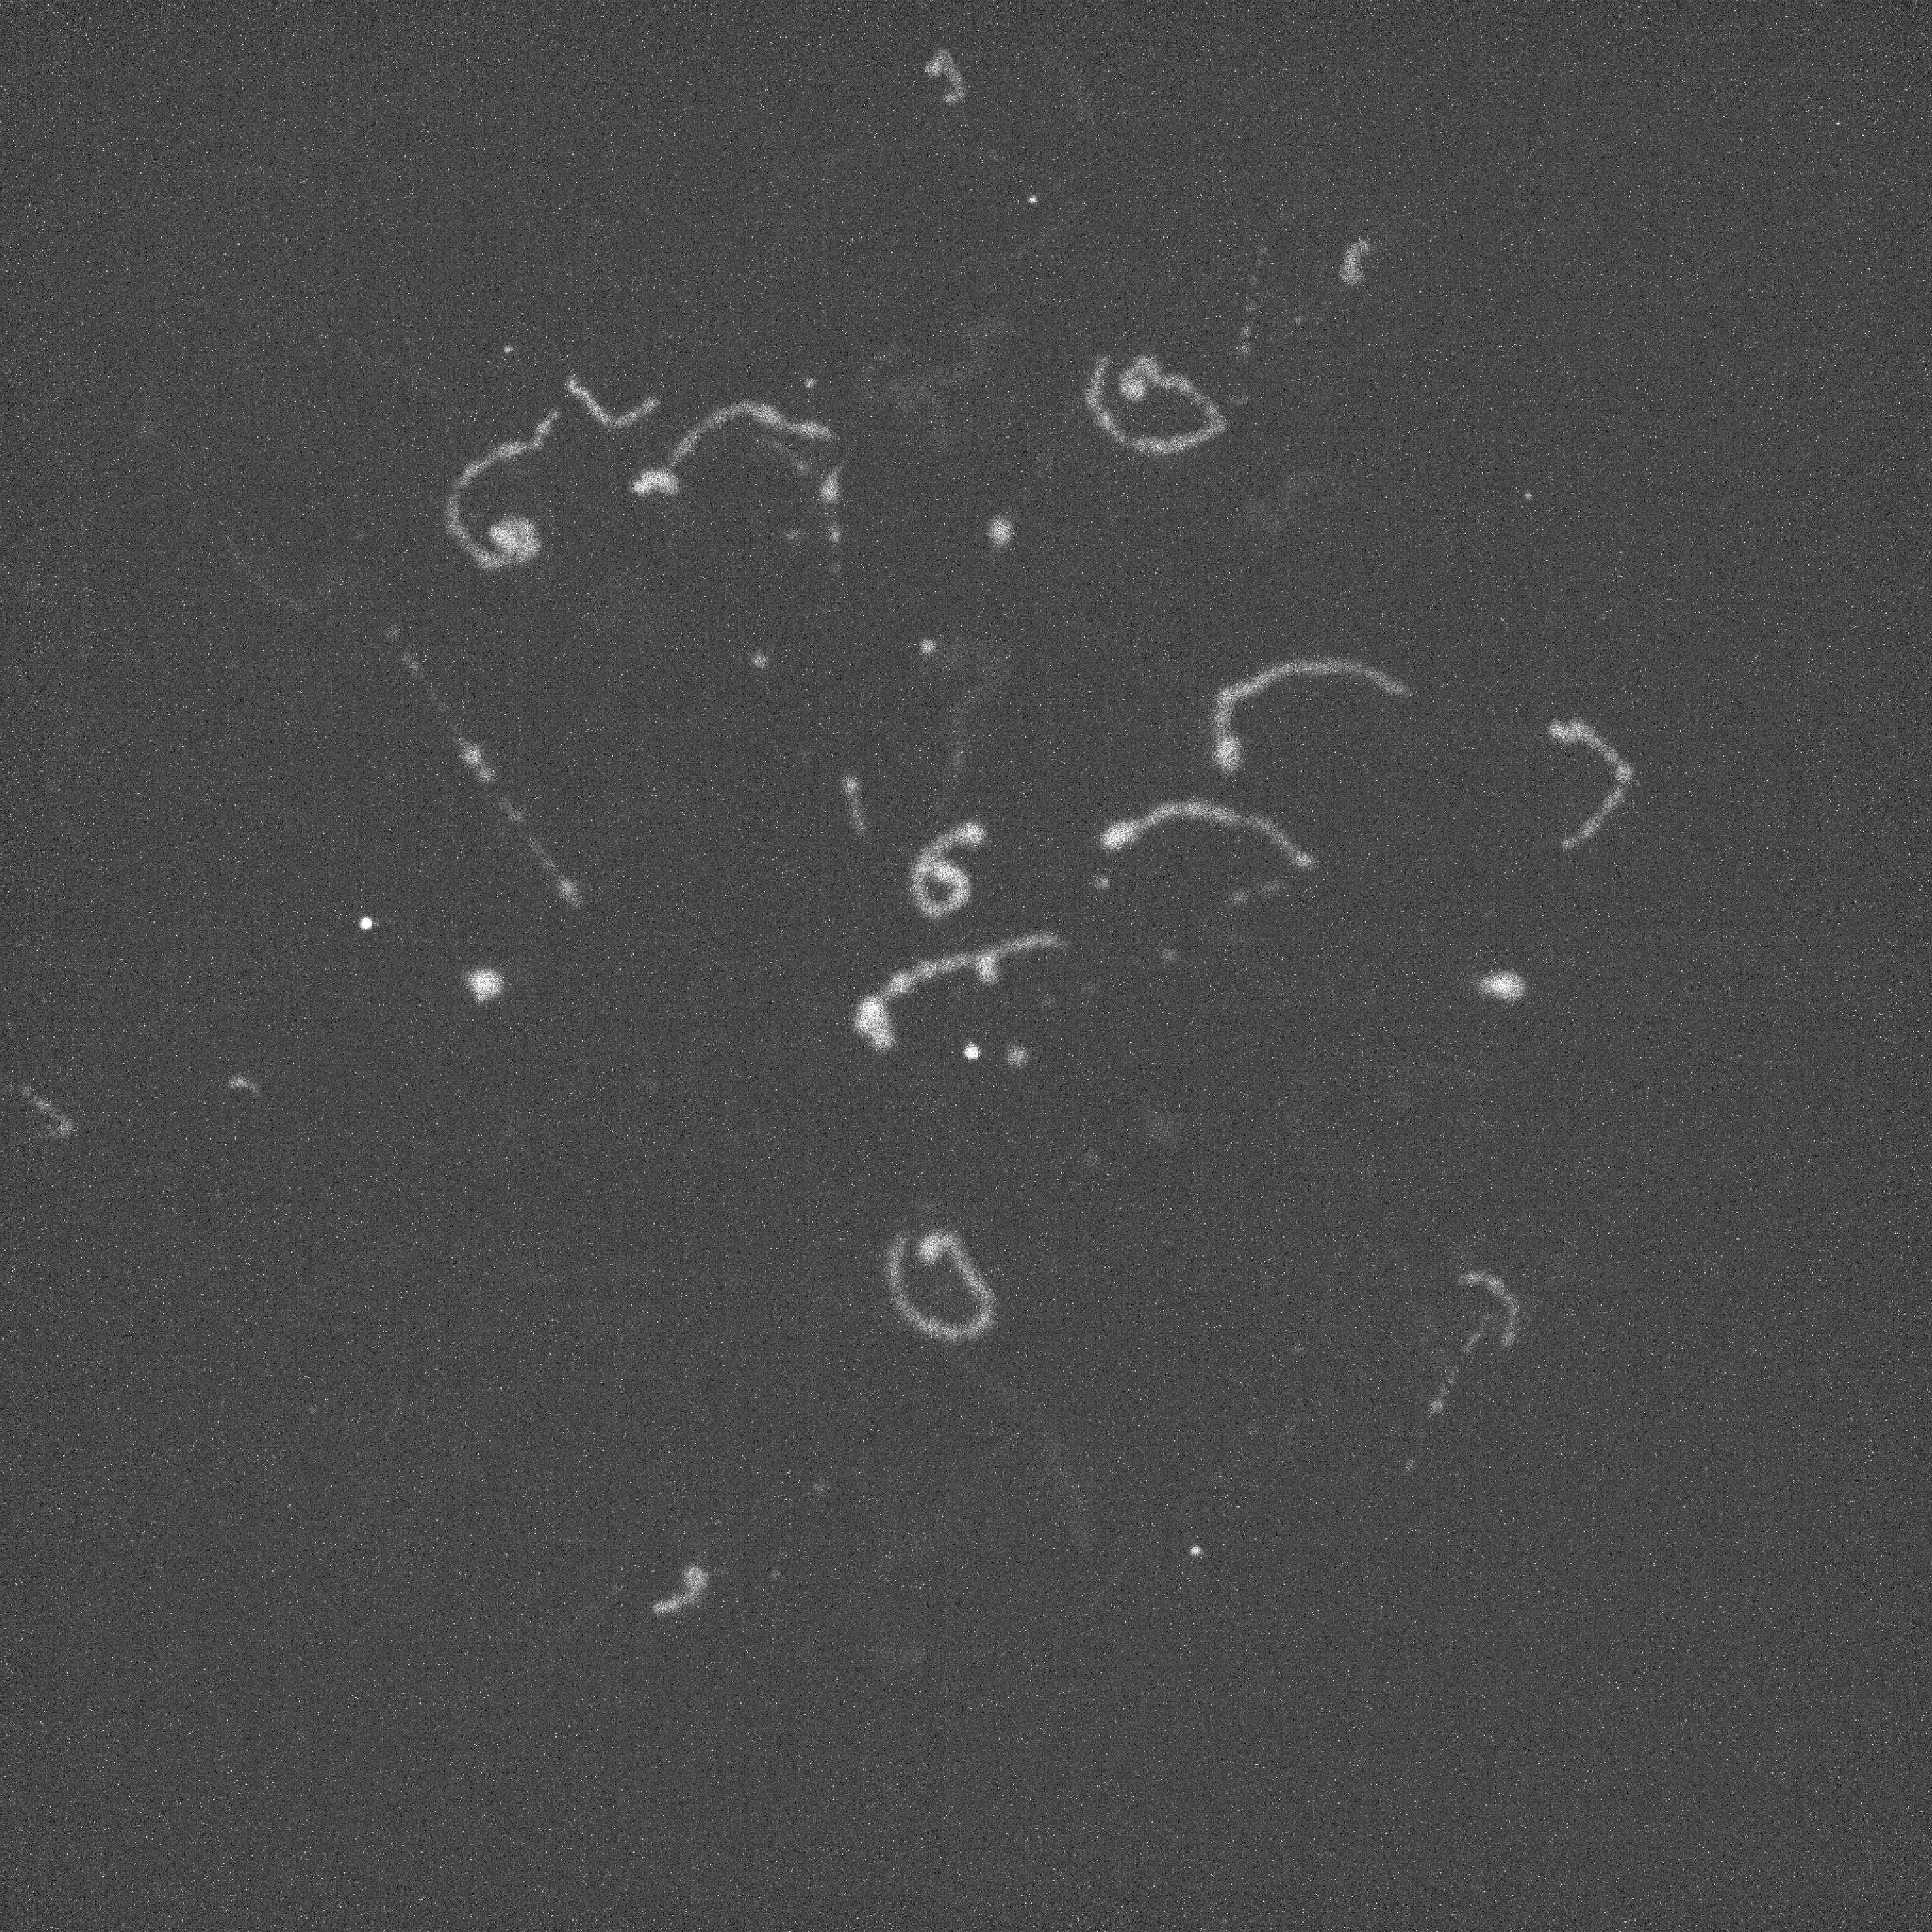
\includegraphics[width=0.4\textwidth]{image_files/494-0005.pdf}
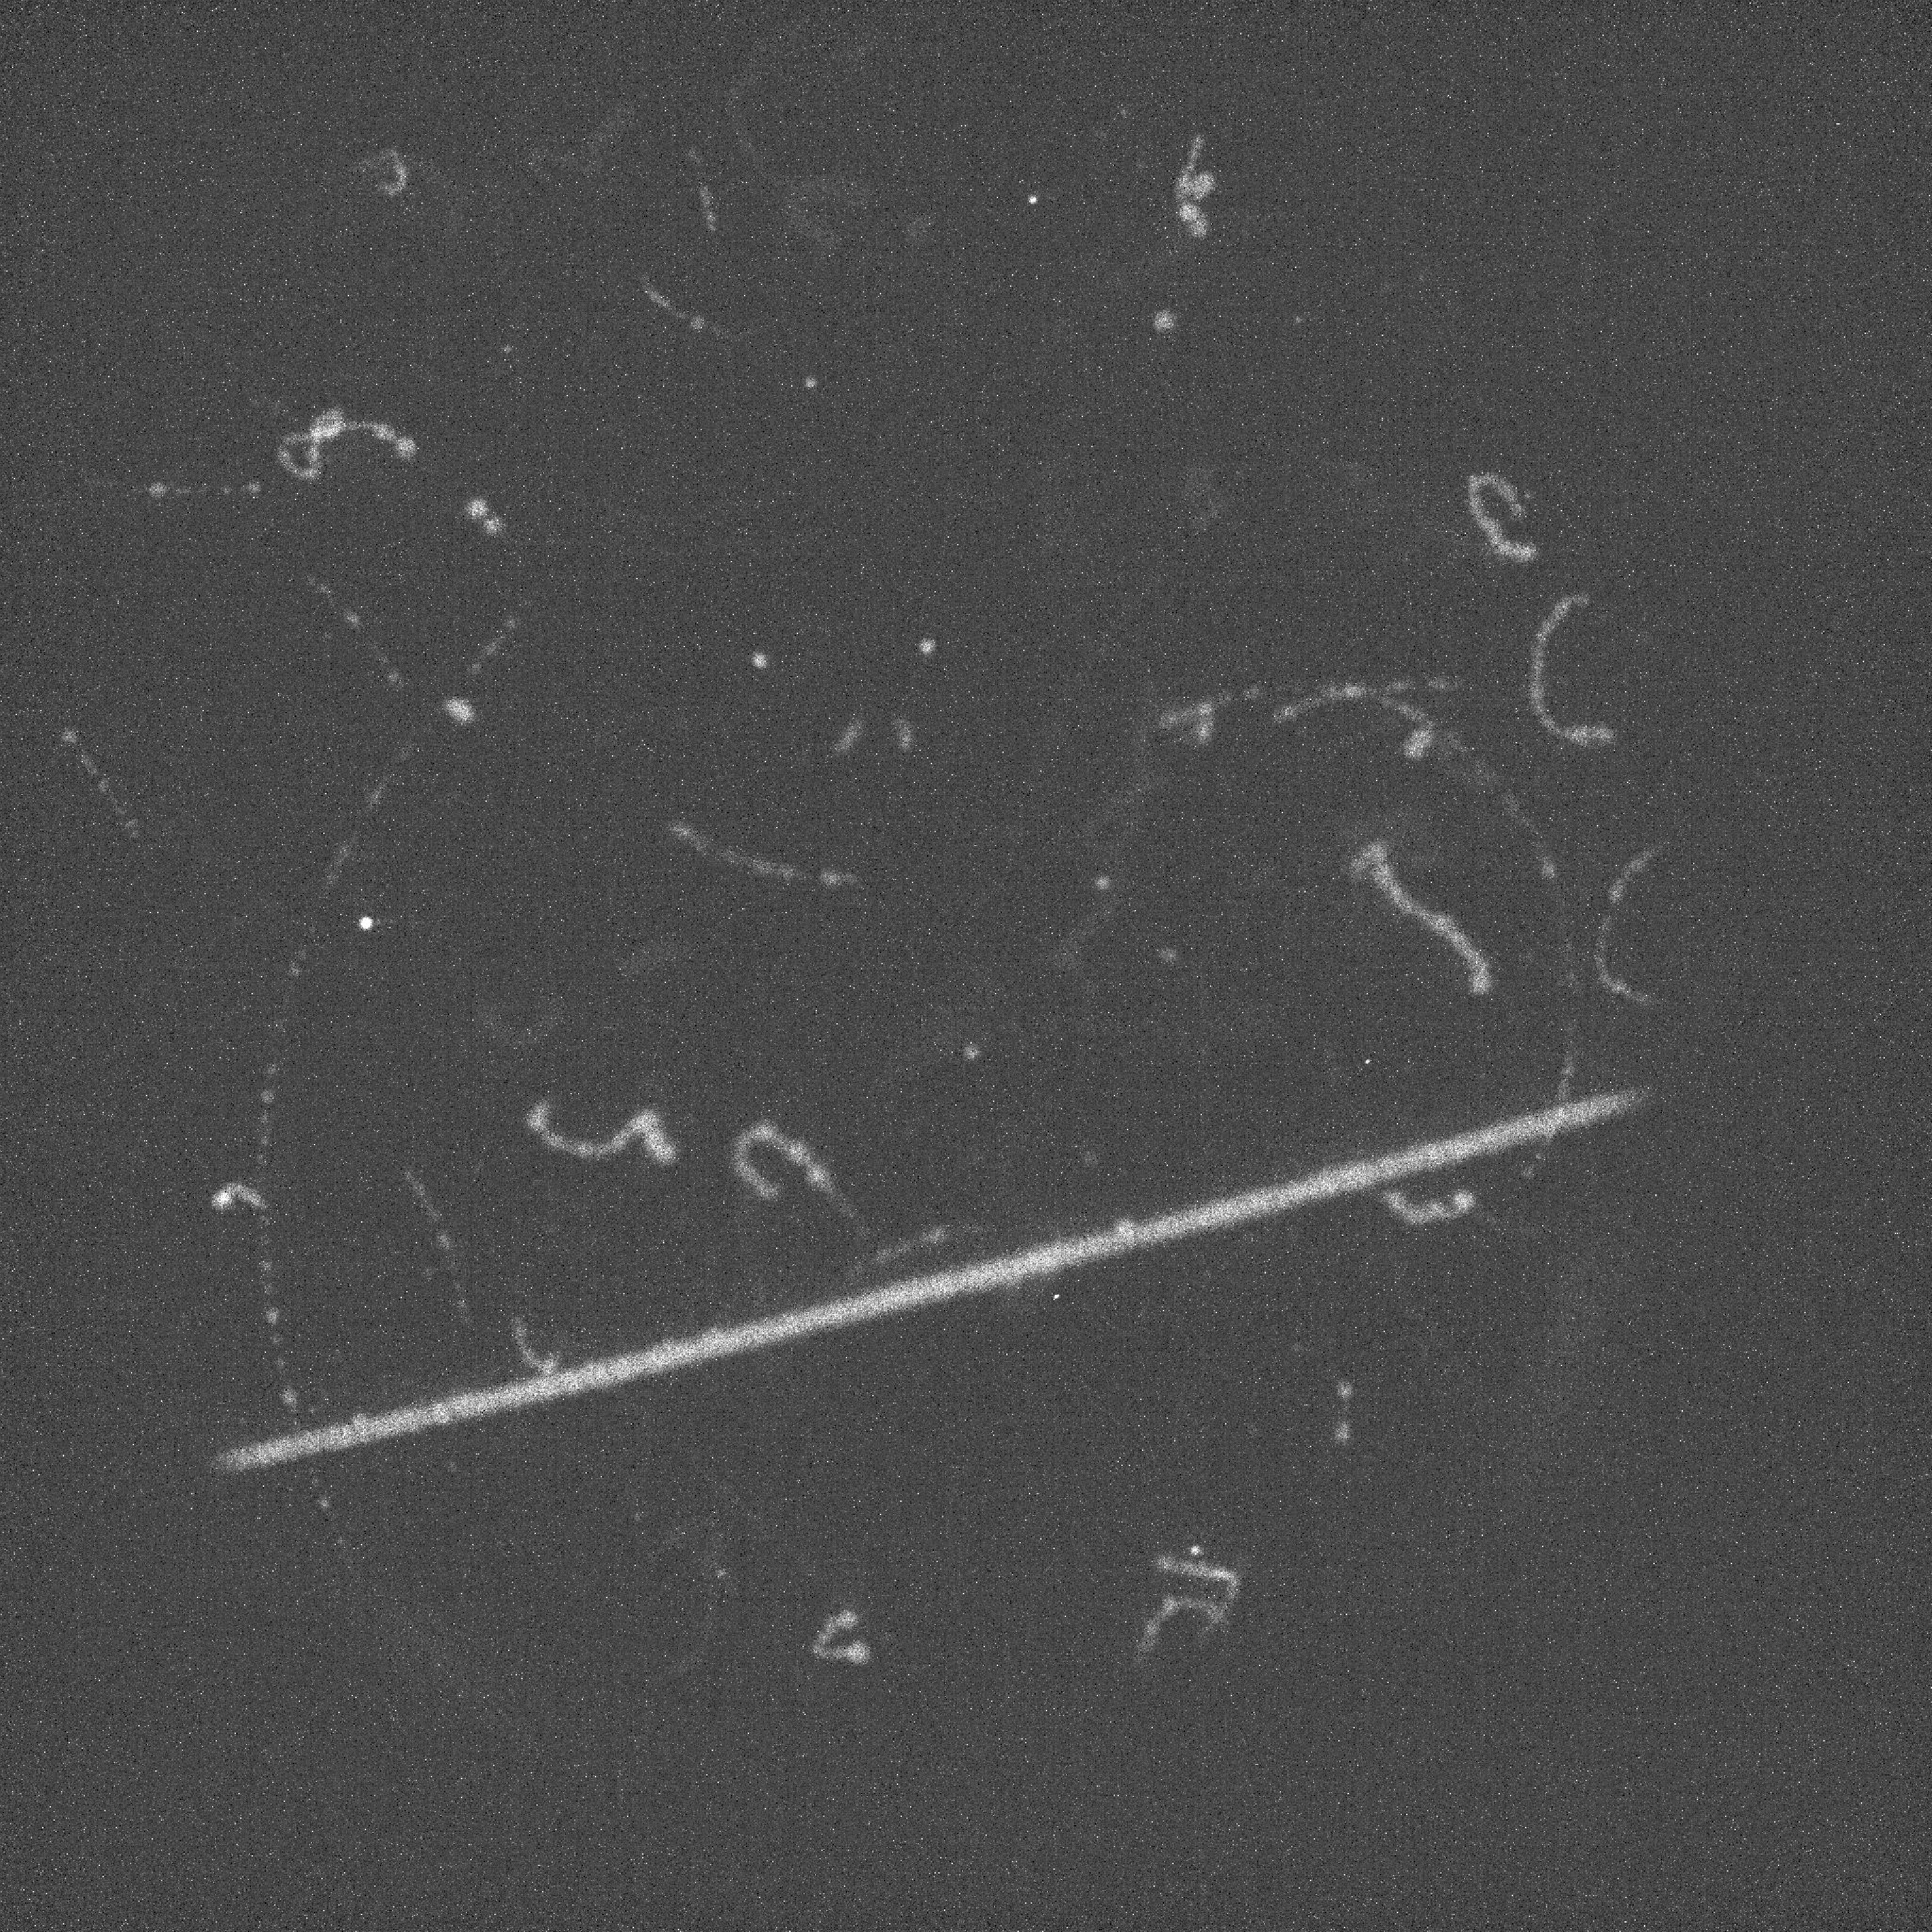
\includegraphics[width=0.4\textwidth]{image_files/494-0001.pdf}
\caption{Images acquired by the ORANGE prototype.} \label{fig_run_494}
\end{figure}

As these images do not have a fundamental truth, it is not possible to determine which filters have the best performance, as well as their respective parameters in a optimal case. \textcolor{red}{cuidado aqui pois com dados reais talvez seja possível avaliar sim qual o "melhor" filtro}

The proposal is to develop a simulation environment where we can evaluate any filtering technique, choosing the best parameters and using them in a real environment. \textcolor{red}{parece que nossa proposta é propor uma simulação enquanto estamos usando a simulação da colaboração}
%%%%%%%%%%%%%%%%%%%%%%%%%%%%%%%%%%%%%%%%%%%%%%
\subsection{Analysis methodology}
%%%%%%%%%%%%%%%%%%%%%%%%%%%%%%%%%%%%%%%%%%%%%%








% \chapter{Literature Review}
% \label{chap:litrev}


% \section{Convolutional Neural Networks (CNN)}

% \section{CNN for signal-background classification in Particle Physics}


%%%%%%%%%%%%%%%%%%%%%%%%%%%%%%%%%%%%%%%%%%%%%%%%%%%%
\chapter{Revisão Bibliográfica}

\section{Formulação matemática do problema de denoising}

O problema de restauração de imagens consiste em recuperar uma imagem ideal $x$ a partir de uma observação degradada $y$. Em sistemas reais de aquisição, o processo de formação da imagem pode ser descrito de forma geral por
\begin{equation}
y = Hx + n,
\end{equation}
onde $H$ representa o operador do sistema de aquisição e $n$ corresponde ao ruído introduzido durante o processo de medição \cite{bertero1998inverse}. No caso particular de denoising, assume-se frequentemente $H = I$, resultando em
\begin{equation}
y = x + n.
\end{equation}

O objetivo consiste então em estimar a imagem verdadeira $x$ a partir da observação $y$. Esse problema é geralmente mal-posto, pois pequenas perturbações na observação podem produzir grandes variações na solução \cite{hadamard1902problemes}. Para lidar com essa dificuldade, métodos de restauração são tipicamente formulados como problemas de otimização regularizados,
\begin{equation}
\hat{x}
=
\arg\min_x
\left(
\|y-x\|_2^2 + \lambda R(x)
\right),
\end{equation}
onde $R(x)$ representa um termo de regularização que incorpora conhecimento \textit{a priori} sobre a estrutura da imagem, e $\lambda$ controla o compromisso entre fidelidade aos dados e regularização.

Uma interpretação alternativa pode ser obtida por meio de uma formulação Bayesiana \cite{jaynes2003probability}. Nesse contexto, busca-se a estimativa \textit{Maximum a Posteriori} (MAP),
\begin{equation}
\hat{x} = \arg\max_x P(x|y).
\end{equation}
Aplicando o teorema de Bayes,
\begin{equation}
P(x|y) \propto P(y|x)P(x),
\end{equation}
e assumindo ruído gaussiano aditivo,
\begin{equation}
P(y|x) \propto
\exp\left(-\frac{1}{2\sigma^2}\|y-x\|_2^2\right),
\end{equation}
obtém-se novamente a formulação variacional
\begin{equation}
\hat{x}
=
\arg\min_x
\left(
\|y-x\|_2^2 + \lambda R(x)
\right),
\end{equation}
na qual o termo de regularização pode ser interpretado como o negativo do logaritmo do prior,
\begin{equation}
R(x) = -\log P(x).
\end{equation}

Em aplicações científicas, o problema torna-se particularmente desafiador devido à baixa relação sinal-ruído (SNR) e à esparsidade espacial do sinal. Em muitas situações experimentais, apenas uma pequena fração dos pixels contém informação útil, enquanto a maior parte da imagem corresponde a fundo ruidoso. Esse cenário é especialmente relevante em imagens contendo estruturas finas, como traços de partículas, filamentos ou bordas de baixa intensidade.

\section{Métodos clássicos de denoising}

Diversas abordagens clássicas foram desenvolvidas para resolver o problema de denoising. Um dos primeiros avanços importantes foi o método de \textit{wavelet shrinkage} proposto por Donoho \cite{donoho1995denoising}. Nesse método, a imagem é representada em uma base wavelet e os coeficientes de pequena magnitude são eliminados por limiarização,
\begin{equation}
\hat{w}_i =
\begin{cases}
w_i - \tau, & |w_i| > \tau,\\
0, & |w_i| \le \tau,
\end{cases}
\end{equation}
onde $\tau$ é um limiar associado ao nível de ruído.

Outro método amplamente utilizado é o \textit{Non-Local Means} (NLM), introduzido por Buades et al. \cite{buades2005nonlocal}. Nesse algoritmo, o valor estimado de um pixel é obtido como média ponderada de pixels pertencentes a regiões semelhantes da imagem,
\begin{equation}
\hat{x}(i)
=
\frac{1}{Z_i}
\sum_j
\exp
\left(
-\frac{\|P_i-P_j\|^2}{h^2}
\right)
y(j),
\end{equation}
onde $P_i$ representa o \textit{patch} centrado no pixel $i$, $h$ controla a intensidade da filtragem e $Z_i$ é um fator de normalização.

Um avanço significativo foi obtido com o método BM3D proposto por Dabov et al. \cite{dabov2007bm3d}, que combina busca de regiões semelhantes com filtragem em domínios transformados tridimensionais. Esse método permaneceu por muitos anos como uma das principais referências em denoising clássico.

No contexto variacional, um modelo amplamente utilizado é o de \textit{Total Variation} (TV), proposto por Rudin, Osher e Fatemi \cite{rudin1992tv},
\begin{equation}
E(x)
=
\|x-y\|_2^2 + \lambda \|\nabla x\|_1.
\end{equation}
Esse modelo promove suavização em regiões homogêneas enquanto preserva descontinuidades importantes da imagem, como bordas e transições abruptas.

Muitos desses métodos podem ser interpretados como processos de difusão não linear. Um exemplo clássico é a equação de difusão anisotrópica proposta por Perona e Malik \cite{perona1990scale},
\begin{equation}
\frac{\partial x}{\partial t}
=
\nabla \cdot
\left(
c(|\nabla x|)\nabla x
\right),
\end{equation}
na qual a função $c(\cdot)$ modula a intensidade da difusão de acordo com a magnitude do gradiente, permitindo suavizar regiões homogêneas sem degradar excessivamente as bordas.

Apesar de sua eficácia em imagens naturais, esses métodos apresentam limitações quando aplicados a imagens científicas extremamente ruidosas ou contendo estruturas muito finas, pois o processo de suavização pode remover componentes de baixa intensidade que ainda carregam informação física relevante.

\section{Representações esparsas}

Uma abordagem alternativa para o problema de denoising baseia-se no conceito de representação esparsa. Nesse contexto, assume-se que a imagem pode ser representada como combinação linear de poucos elementos de um dicionário,
\begin{equation}
x = D\alpha,
\end{equation}
onde $D$ representa uma base ou dicionário e $\alpha$ é um vetor esparso de coeficientes.

O problema de denoising pode então ser formulado como
\begin{equation}
\hat{\alpha}
=
\arg\min_\alpha
\left(
\|y-D\alpha\|_2^2 + \lambda \|\alpha\|_1
\right).
\end{equation}
Essa formulação favorece soluções nas quais apenas um pequeno número de coeficientes é diferente de zero. A reconstrução final da imagem é então dada por $\hat{x}=D\hat{\alpha}$.

Essa abordagem foi explorada por Elad e Aharon \cite{elad2006ksvd} no contexto de \textit{dictionary learning}, utilizando o algoritmo K-SVD para aprender o dicionário diretamente a partir dos dados. Representações esparsas são particularmente adequadas para sinais contendo estruturas geométricas simples, como bordas, linhas ou filamentos \cite{starck2010sparse}. Em imagens científicas nas quais o sinal aparece como trajetórias finas sobre fundo ruidoso, essa hipótese de esparsidade torna-se especialmente natural.

Do ponto de vista matemático, esse tipo de formulação estabelece uma ponte entre o problema de denoising e problemas inversos esparsos, nos quais a solução procurada apresenta suporte espacial reduzido ou representação compacta em uma base apropriada.

\section{Deep learning para restauração de imagens}

Nos últimos anos, redes neurais profundas passaram a desempenhar papel central em problemas de restauração de imagens \cite{goodfellow2016deep}. Nesse contexto, a imagem restaurada é obtida por meio de uma função paramétrica
\begin{equation}
\hat{x} = f_\theta(y),
\end{equation}
onde $f_\theta$ representa uma rede neural convolucional parametrizada por $\theta$.

Os parâmetros da rede são ajustados minimizando uma função de perda definida sobre um conjunto de treinamento,
\begin{equation}
\mathcal{L}(\theta)
=
\sum_i
\|f_\theta(y_i)-x_i\|_2^2,
\end{equation}
onde $(y_i,x_i)$ representa um par formado por imagem ruidosa e sua respectiva referência.

Uma abordagem particularmente eficaz consiste em treinar a rede para estimar diretamente o ruído presente na imagem, resultando em
\begin{equation}
\hat{x} = y - f_\theta(y).
\end{equation}
Esse princípio é utilizado em métodos como o DnCNN \cite{zhang2017dncnn}, que demonstraram desempenho superior a diversas técnicas clássicas.

Além disso, trabalhos recentes mostraram que redes convolucionais podem ser interpretadas como versões aprendidas de processos iterativos de difusão \cite{chen2017reaction}. Em uma formulação simplificada, a atualização entre duas camadas pode ser escrita como
\begin{equation}
x_{k+1}
=
x_k +
\sum_i
K_i^T
\phi_i(K_i x_k),
\end{equation}
onde $K_i$ são filtros convolucionais e $\phi_i$ são funções não lineares aprendidas. Essa interpretação conecta arquiteturas profundas com modelos variacionais clássicos e equações de difusão não linear.

A principal vantagem desses métodos em relação às abordagens tradicionais está na capacidade de aprender, diretamente a partir dos dados, regularidades estatísticas e geométricas específicas do domínio de aplicação. Em vez de impor explicitamente uma regularização fixa, a rede aprende um regularizador implícito ajustado ao tipo de imagem considerado.

\section{Arquiteturas multi-escala e aplicação a imagens esparsas}

Entre as arquiteturas utilizadas em restauração de imagens, destaca-se a U-Net proposta por Ronneberger et al. \cite{ronneberger2015unet}. Essa arquitetura é composta por um \textit{encoder}, responsável por extrair representações progressivamente mais abstratas da imagem, e um \textit{decoder}, responsável por reconstruir a imagem final.

Cada camada convolucional pode ser representada por
\begin{equation}
F_{l+1}
=
\sigma(W_l * F_l + b_l),
\end{equation}
onde $W_l$ representa o kernel de convolução, $b_l$ é o viés da camada e $\sigma$ é uma função de ativação não linear.

Uma característica fundamental da U-Net é a presença de \textit{skip connections},
\begin{equation}
F_l^{dec}
=
\mathrm{concat}(F_l^{enc},F_l^{up}),
\end{equation}
que conectam diretamente mapas de características do encoder aos níveis correspondentes do decoder. Essas conexões permitem preservar detalhes espaciais de alta resolução durante o processo de reconstrução.

Arquiteturas multi-escala são particularmente adequadas para imagens contendo estruturas em diferentes resoluções espaciais. Em muitas aplicações científicas, o sinal útil aparece como estruturas lineares ou filamentares muito localizadas, imersas em fundo ruidoso. Nesse cenário, torna-se essencial combinar informação local de alta resolução com contexto global, de modo a distinguir estruturas reais de flutuações estatísticas.

Em detectores de partículas com leitura óptica, como aqueles utilizados no experimento CYGNO, o sinal útil aparece como trajetórias finas que ocupam apenas uma pequena fração da imagem. Esse cenário pode ser interpretado como um caso particular de problema inverso esparso, no qual a imagem verdadeira contém um conjunto reduzido de estruturas relevantes sobre um fundo amplamente dominado por ruído. A aplicação de arquiteturas do tipo U-Net torna-se, portanto, particularmente promissora, pois sua estrutura multi-escala e suas conexões de atalho favorecem a preservação de traços finos ao mesmo tempo em que reduzem componentes espúrios do fundo.

\section{Lacunas na literatura e motivação do trabalho}

A evolução das técnicas de denoising mostra um progresso consistente desde abordagens baseadas em transformadas e regularização variacional até métodos baseados em aprendizado profundo. Técnicas clássicas, como \textit{wavelet shrinkage}, NLM, BM3D e Total Variation, oferecem soluções matematicamente bem fundamentadas para a redução de ruído, enquanto modelos baseados em representações esparsas e redes neurais profundas ampliaram significativamente a capacidade de adaptação a diferentes tipos de imagem.

Apesar desses avanços, grande parte da literatura concentra-se em imagens naturais, biomédicas ou em cenários nos quais o sinal útil ocupa uma fração substancial da imagem. Em contraste, diversas aplicações científicas produzem imagens com propriedades bastante distintas, caracterizadas por: (i) baixa relação sinal-ruído; (ii) ocupação espacial extremamente reduzida; e (iii) presença de estruturas finas, muitas vezes lineares ou filamentares, de baixa intensidade.

Esse cenário é particularmente relevante em detectores de partículas com leitura óptica, nos quais os eventos físicos de interesse aparecem como traços esparsos em imagens de alta resolução. Nesses casos, métodos de denoising excessivamente suaves podem degradar ou até eliminar a estrutura do traço, comprometendo etapas posteriores de reconstrução, identificação e classificação de eventos. Por outro lado, métodos insuficientemente seletivos podem preservar grande parte do ruído de fundo, limitando o ganho efetivo em SNR.

Embora arquiteturas profundas tenham demonstrado excelente desempenho em tarefas gerais de restauração de imagens, ainda há relativamente poucos estudos focados em imagens esparsas contendo trajetórias de partículas adquiridas em detectores ópticos. Em particular, permanece aberta a investigação de como arquiteturas do tipo U-Net podem ser exploradas para melhorar a SNR sem comprometer a morfologia dos traços detectados.

Nesse contexto, o presente trabalho é motivado pela necessidade de desenvolver e avaliar uma abordagem de denoising especificamente voltada para imagens esparsas de traços de partículas, utilizando como base dados simulados com verdade conhecida para treinamento supervisionado. A escolha de uma arquitetura do tipo U-Net se justifica por sua capacidade de combinar informação multi-escala e preservação de detalhes espaciais, características fundamentais para esse tipo de aplicação. Espera-se, com isso, obter imagens com maior qualidade para etapas posteriores de análise, mantendo a integridade geométrica e fotométrica das estruturas associadas aos eventos físicos de interesse.





%%%%%%%%%%%%%%%%%%%%%%%%%%%%%%%%%%%%%%%%%%%%%%%%%%%%






























\chapter{CYGNO Experiment}
\label{chap:cygnoexp}

\section{Motivation}

\section{Technology}
\subsection{TPC}
\subsection{GEM}
\subsection{Optical Readout}


\section{Apparatus}


%-----------------------------------------------

%-----------------------------------------------
\chapter{Methodology}
\label{chap:methodology}
%-----------------------------------------------
In this section, the methodology developed to evaluate the impact of filtering as a preprocessing technique on images from the LeMon detector will be discussed. The process can be divided into two parts, the first one has as main objective, to select optimal parameters for the filters used. 
Such selection is only possible from the use of simulation images provided by the collaboration, since in this case the output is known and an adequate efficiency evaluation metric was chosen to measure the performance of the algorithms. For the second part, once the optimal filter parameters have been chosen, their performance in the reconstruction algorithm as a whole will be evaluated, comparing output variables such as energy and processing time. 

The main objective of this analysis is to verify the real impact of the use of filters in relation to the algorithm currently used by the CYGNO Experiment.


\section{CYGNO's Experiment reconstruction algorithm overview}
The version of the reconstruction algorithm used in this work is shown in the flowchart of figure \ref{recoflow}.

\begin{figure}[H]
\centering
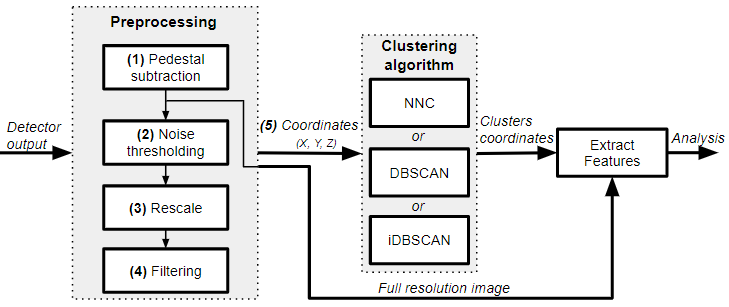
\includegraphics[width=0.7\textwidth]{image_files/fluxgram_algorithm.PNG}
\caption{Reconstruction algorithm flowchart \ref{baracchini2020density}}
\label{recoflow}
\end{figure}

The detector output images are sent to a set of algorithms, which preprocess them. This preprocessing is defined by the following steps:

\begin{itemize}
    \item Pedestal subtraction: The output image of the detector can be described from the composition of the result of the interaction of the particles inside the detector and also from the portion of electronic noise, originated during the capture of events by the camera, inside the detector. The purpose of pedestal removal is to subtract from the image the average effect of noise at each pixel. For this to be possible, the average noise value of each pixel is obtained by capturing images with the camera obstructed, being possible to collect, in addition to the average value, the probability distribution of each one.
    
    \item{Noise thresholding}
    Once the expected noise value has been removed for each pixel, the next step consists of a threshold on the same pixels based on the noise information extracted from images with the camera obstructed. This threshold is based on the standard deviation of camera noise, and its main objective is to filter the pixels that had an intensity value greater than a number n times the standard deviation value of each pixel. Currently, this value is close to 1.3 times the standard deviation of noise at each pixel.
    
    \item{Rescale} 
    Also known as rebinding, the rescaling process consists of re-scaling the image in order to reduce its size. The scale factor used by algorithm is 4, so for a input image of size 2048x2048 becames a 512x512 image. The main objective of this procedure is to reduce the number of pixels that will be sent to the clustering algorithm, aiming to reduce the computational cost of the process as a whole.
    
    \item{Filtering}
    After rescaling, a median filter is applied replacing the pixel value with the median of its value, along with that of its neighbors. The number of neighbors used at this step is 16 (4x4 window).
\end{itemize}

After the preprocessing step, the filtered pixels, together with their respective intensity values, are sent to a clustering algorithm to form clusters of particles. The algorithm used in this version uses idbscan, which presents better results compared to other already tested algorithms such as DBSCAN and NNC \ref{baracchini2020density}.

Finally, once the clusters are extracted, their features are calculated to understand the interactions that occurred in the detector. The main one used in this work is the energy, proportional to the sum of intensities of the pixels belonging to the cluster found. From the scale of conversion of the pixel intensity value to the number of photo electrons, the particle energy value can be recovered.

\section{Proposed reconstruction algorithm}

Understanding better about the energy reconstruction process, it is possible to think of improvement strategies for the algorithm. The purpose of the present work is, first, to propose a different way from the one used for pixel selection and, in addition, to develop a benchmarking environment, to verify the advantages and disadvantages of each approach.

The idea initially proposed is based on the optimization of the selection of pixels after the threshold step. It is expected that the maximum energy that can be reconstructed is obtained when only the pixels that are actually part of the event are sent to the clustering algorithm. Therefore, improving this process impacts on improvements in the reconstruction process. 

Analyzing the formation of images, from the interaction of the event inside the detector, to the output generated by the camera, the biggest problem of the pixel selection step can be seen, the electronic noise introduced by the image capture process. The inserted noise varies the intensity value of the pixels, directly influencing the value of the reconstructed energy. This variation can be characterized in the frequency domain, by components located at higher frequencies, which can be attenuated by image filtering techniques. Filtering performed in the frequency domain, are interesting for presenting linear characteristics when represented in the space domain, and generally have a lower computational cost. However, not only these can solve this kind of problem, non-linear filters can also be used for noise filtering, in addition to techniques based on machine learning.

The proposed algorithm, composed of a filtering step to attenuate the electronic noise coming from the camera, is shown in figure x. The main changes in relation to the version used by the experiment are:

\begin{itemize}
    \item Filtering after pedestal subtraction: The pedestal subtraction was kept and filtering step are applied to an image with mean noise value of pixels subtracted.
    
    \item Threshold after filtering: Filtering operation can change the image intensity values domain, so the threshold will be applied after filtering.
    
    \item All steps after rescale removed: Once filters and thresholding applied, only rescale was kept, once a filtering process have already been applied.
\end{itemize}

In order to simplify the analyzes performed, no parameter of the clustering algorithm was changed, since the initial premise was that the optimization of the pixel selection process can generate improvements in the energy reconstruction process.

Since the use of filters to improve energy reconstruction has been proposed, it is necessary to define a coherent way to select the parameters of filters and evaluating the performance of these algorithms together with the algorithm used by the experiment currently.

In the next section, the development of the filter parameter selection environment and the evaluation of the algorithms will be discussed.

\section{A pixel selection evaluation environment}

The proposed environment to measure pixel selection techniques for CYGNO reconstruction algorithm is shown in the figure \ref{diagram}. This setup will be used to performance of algorithms evaluation and can also be used to chose optimal parameters for these algorithms.

\begin{figure}[H]
\centering
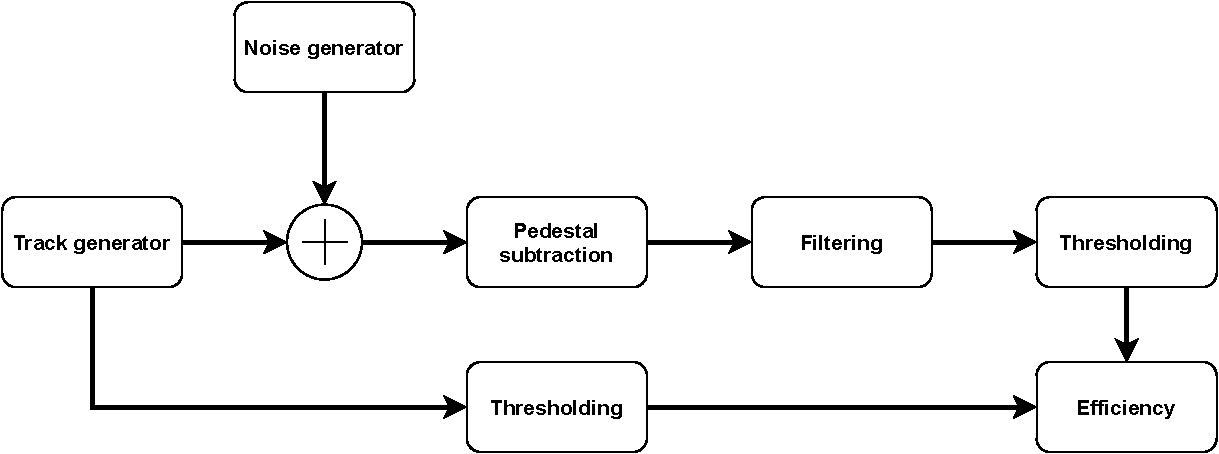
\includegraphics[width=1\textwidth]{image_files/diagrama_dissertacao.pdf}
\caption{Simulation environment}
\label{diagram}
\end{figure}

The fundamental condition for this proposal to work is to know the ground truth of the input image, since this answer is used to determine the efficiency. For this reason, simulation images will be used to define the algorithms and parameters for validation of the proposed methodology.

\subsection{Track generator}
The track generator's main objective is to convert the interactions of the detector particles into images, this step is extremely important, since the closer the generated images are to what is found in practice, the more adjusted to reality this proposal will become. Some attempts to model these interactions have been developed in \ref{lopes2019study} but the CYGNO Experiment has a Monte Carlo based simulation using Geant4 \ref{incerti2010geant4} that was adopted in the development of this work. In the figure \ref{trackgenerator} it's possible to see an example of Electron recoil 60 $keV$ image generated after Geant4 simulation. 
In the image to the side, we have the same image submitted to a threshold of 0, indicating only the pixels that were triggered during the interaction of the particle inside the detector.

\begin{figure}[H]
\centering
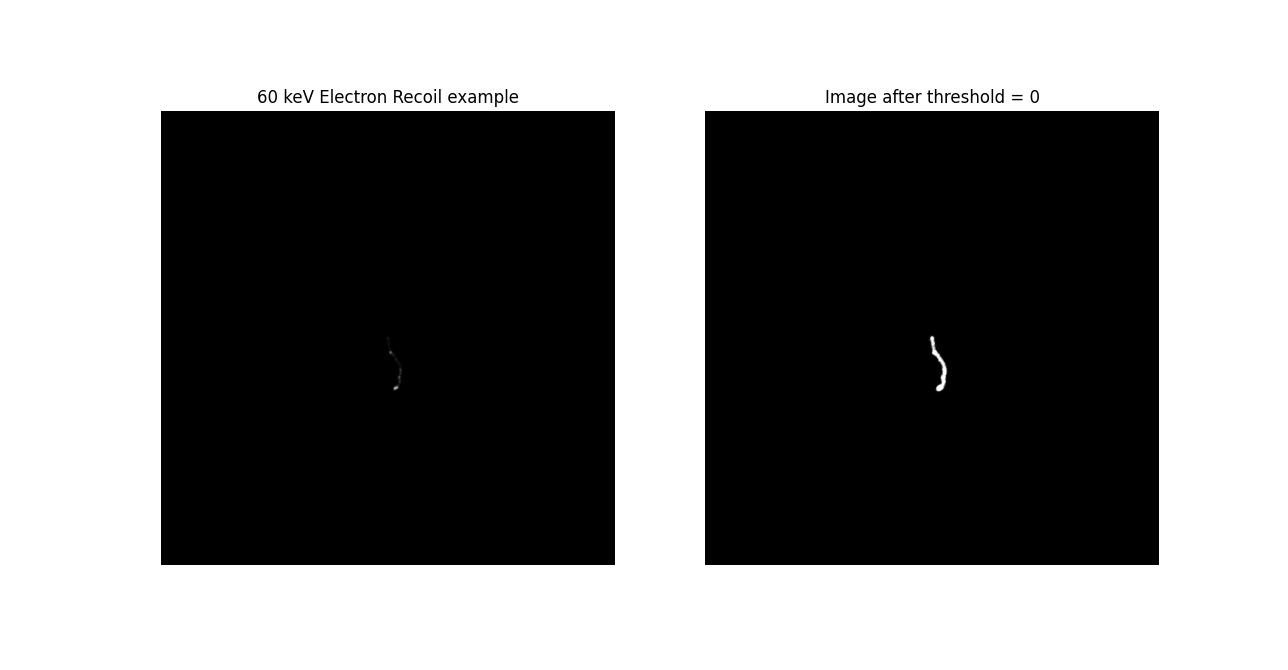
\includegraphics[width=1\textwidth]{image_files/track_generator.png}
\caption{Track generator example}
\label{trackgenerator}
\end{figure}


\subsection{Noise generation}
In order to have an image closer to the reality of the detector in question, we inserted an electronic noise simulator in this environment. A real image can be defined by equation \ref{eq_noise}, where $I_{real}[x,y]$ is the image after noise insertion, $I_{truth}[x,y]$ is the image after track generator and $\eta[x,y]$ is the noise image generated. 

\begin{equation}
    I_{real}[x, y] = I_{truth}[x, y] + \eta[x, y] 
\label{eq_noise}
\end{equation}

An image data-set was collected when the camera lens is turned off, aiming to obtain only the noise portion related to the acquisition electronics. From the intensity distribution of each pixel, assuming that the noise probability distribution is independent for each pixel, a Monte Carlo simulation was used to create a random noise generator with a probability distribution close to real.

An example of this step can be shown in the figure \ref{noise_insertion}.


\begin{figure}[H]
\centering
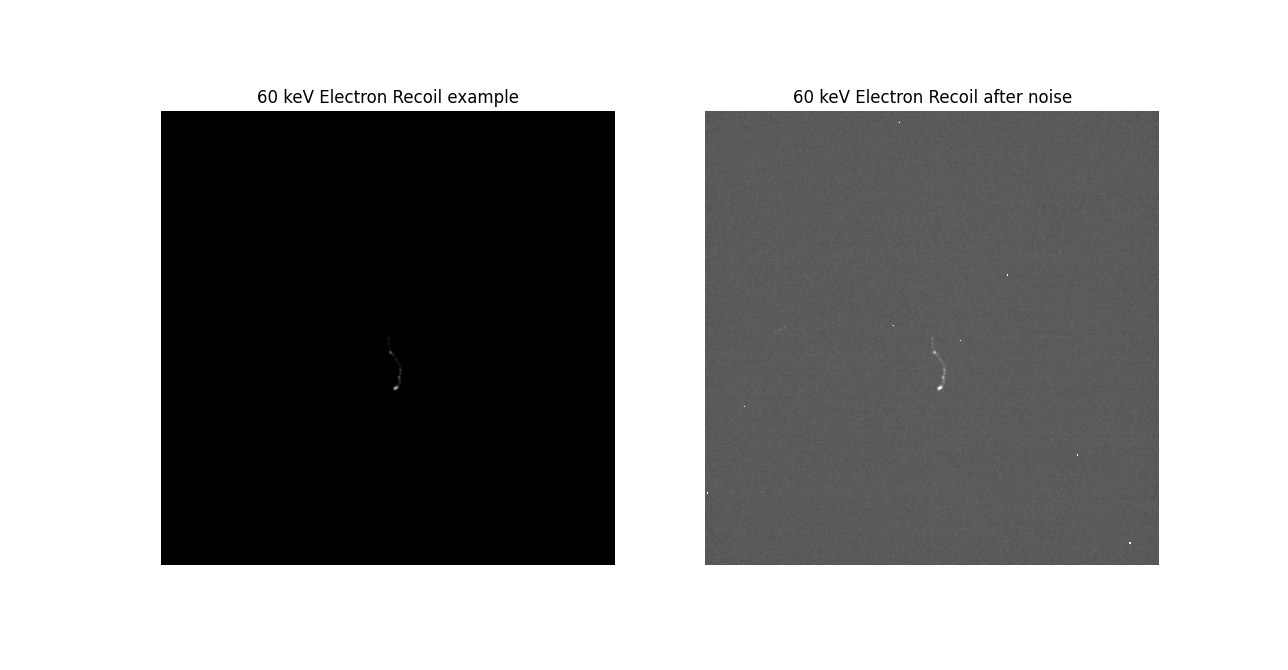
\includegraphics[width=1\textwidth]{image_files/noise_insertion.png}
\caption{Image after noise insertion}
\label{noise_insertion}
\end{figure}



\subsection{Pedestal subtraction}
After to insert noise in images, the pedestal is removed using the mean value of noise for each pixel. An image called a pedmap, containing these values for each pixel, is used in this procedure.

The main idea behind this step, is to try to take to 0, the value of the intensity of the pixels that were not activated by the particle, in the detector. As for the pixels that were activated, remove the noise portion of its value, trying to be as close as possible to the value that it actually should have been, if there was no noise present. 

The pedestal subtraction process can be shown in the figure \ref{pedestal}. First, its possible to see in \ref{hist_img} the histogram of pixels for an image after noise insertion. It's possible to notice that most pixels have an intensity value greater than 0. For the same image intensity histogram, but when pedestal is subtracted, the figure \ref{hist_img_ped} shows that the most part of pixels presents values closer to 0.

\begin{figure}
     \centering
     \begin{subfigure}[b]{0.5\textwidth}
         \centering
         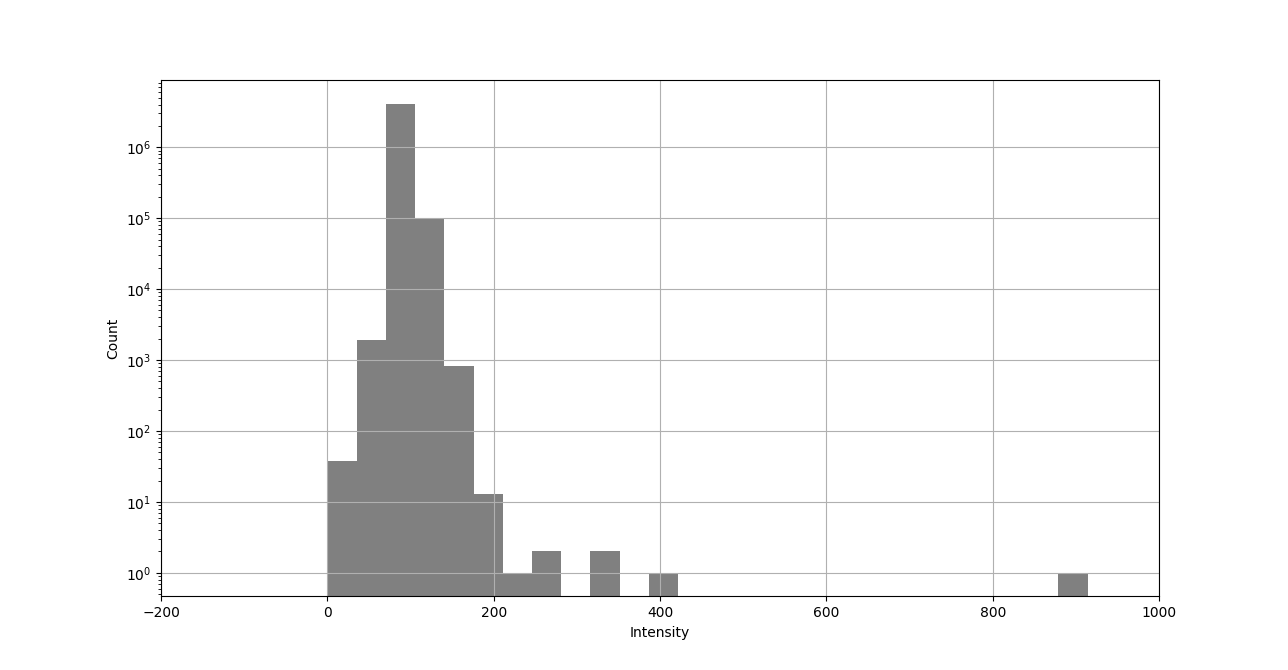
\includegraphics[width=\textwidth]{image_files/noise_before_ped.png}
         \caption{Histogram of intensity of an image before pedestal subtraction}
         \label{hist_img}
     \end{subfigure}
     \hfill
     \begin{subfigure}[b]{0.5\textwidth}
         \centering
         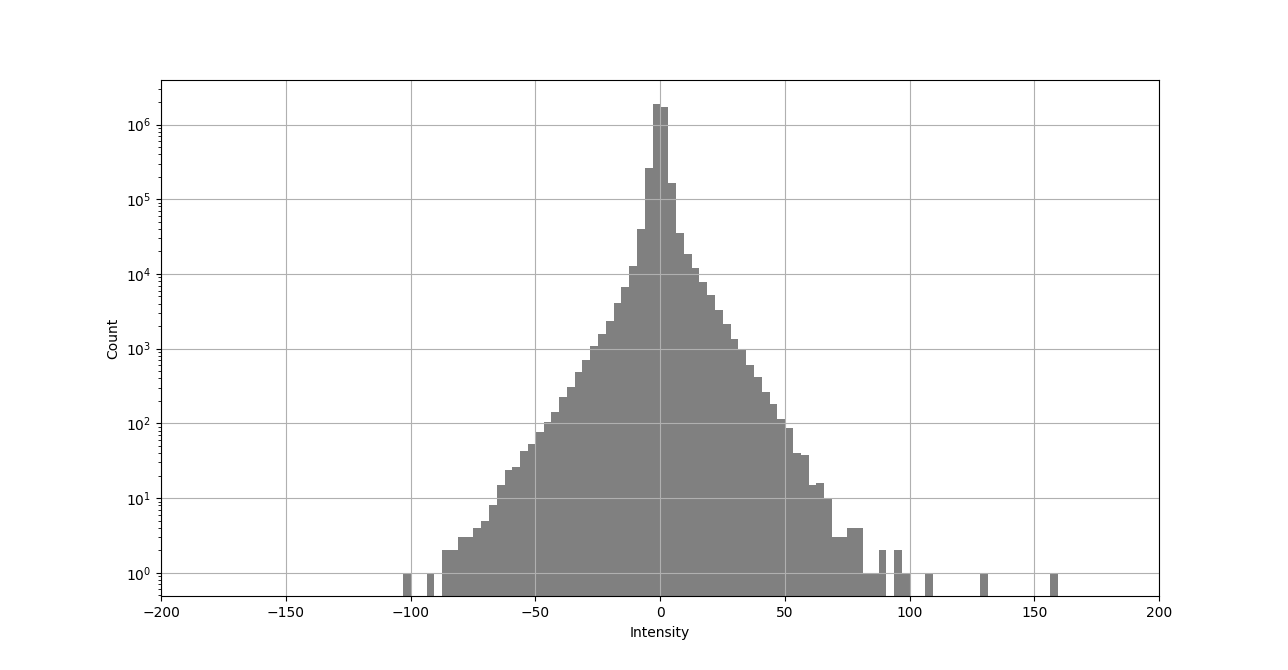
\includegraphics[width=\textwidth]{image_files/noise_after_ped.png}
         \caption{Histogram of intensity of an image after pedestal subtraction}
         \label{hist_img_ped}
     \end{subfigure}
     \label{pedestal}
\end{figure}

An example of image after pedestal subtraction is shown on figure \ref{ped_sub}. When compared this image to the image of figure \ref{noise_insertion}, it's possible to see that some pixel spikes disappear. It's happens because this is a camera effect, bring some pixels specific pixels to very high intensity value. When noise is acquired, these pixels presents these effect that can be got by mean value and removed after pedestal subtraction process.  

\begin{figure}[H]
\centering
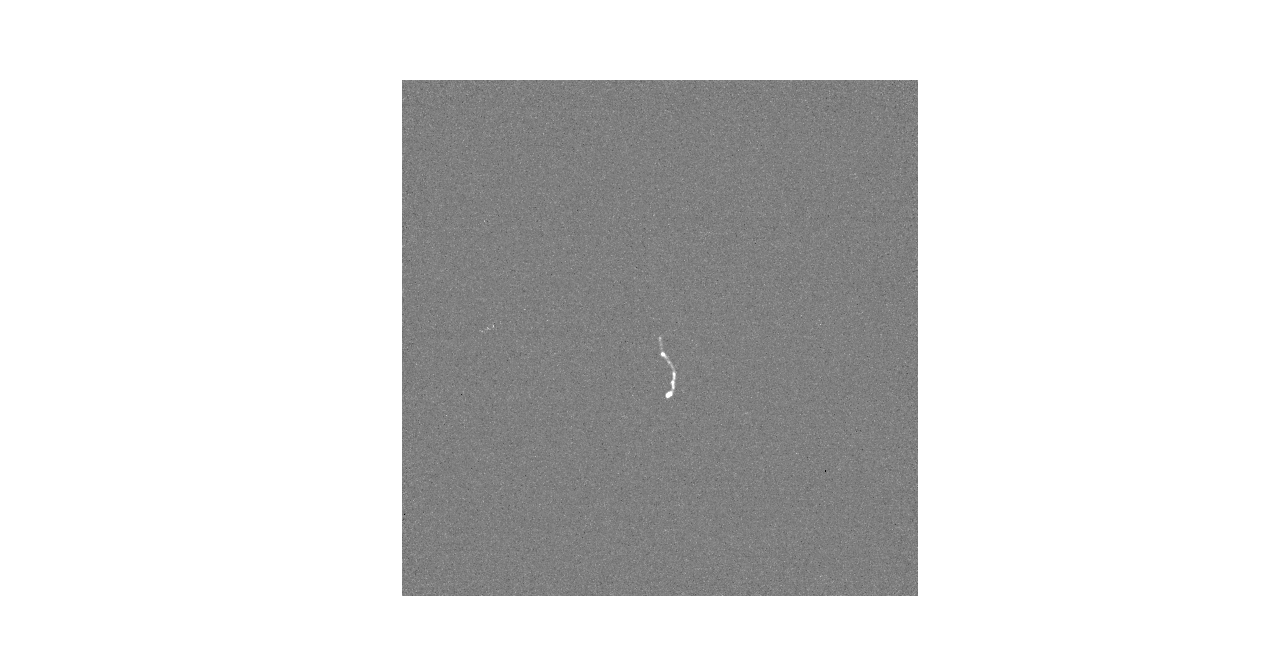
\includegraphics[width=1\textwidth]{image_files/image_after_ped.png}
\caption{Image after pedestal subtraction}
\label{ped_sub}
\end{figure}


\subsection{Filtering}
The filtering process consists of applying digital filters to the images after noise insertion, aiming to improve the pixel selection process, improving the separation of the distributions of pixels that are considered signal and the background pixels, facilitating the threshold step. 
The filters selected to evaluate the proposed work were smoothing filters and a deep learning based pixel selection.

%Smoothing filters are mainly used to reduce noise of an image and for blurring \ref{chaki2018beginner}, and for CYGNO Experiment problem, they are used for reduce the amount of noise on images. \ref{chaki2018beginner} divides smoothing filters into two main types, Smoothing Linear Filters and Order-Statistics Filters.%

\subsubsection{Smoothing filters}

For smoothing filters, the Mean \ref{} and Gaussian \ref{} filters were chosen to represent linear filters and Median filter to represent non linear filters \ref{}. Those techniques will be used in this work. 
The main reason for this choice is the simplicity of the applied transformations, 
since the number of parameters defined for each one is small, in addition to the which facilitate the understanding of the results obtained during the development of the work.

In the figures \ref{mean_example}, \ref{gaussian_example}, \ref{median_example} it's possible to see the effect of filtering in simulation images by changing window parameter for each used filter. The higher the window value, the more the image is blurred, removing the high variations in intensities caused by noise. On the other hand, the characteristics of the particles are also lost, and it is necessary to find an ideal point for this trade-off.


\begin{figure}[H]
\centering
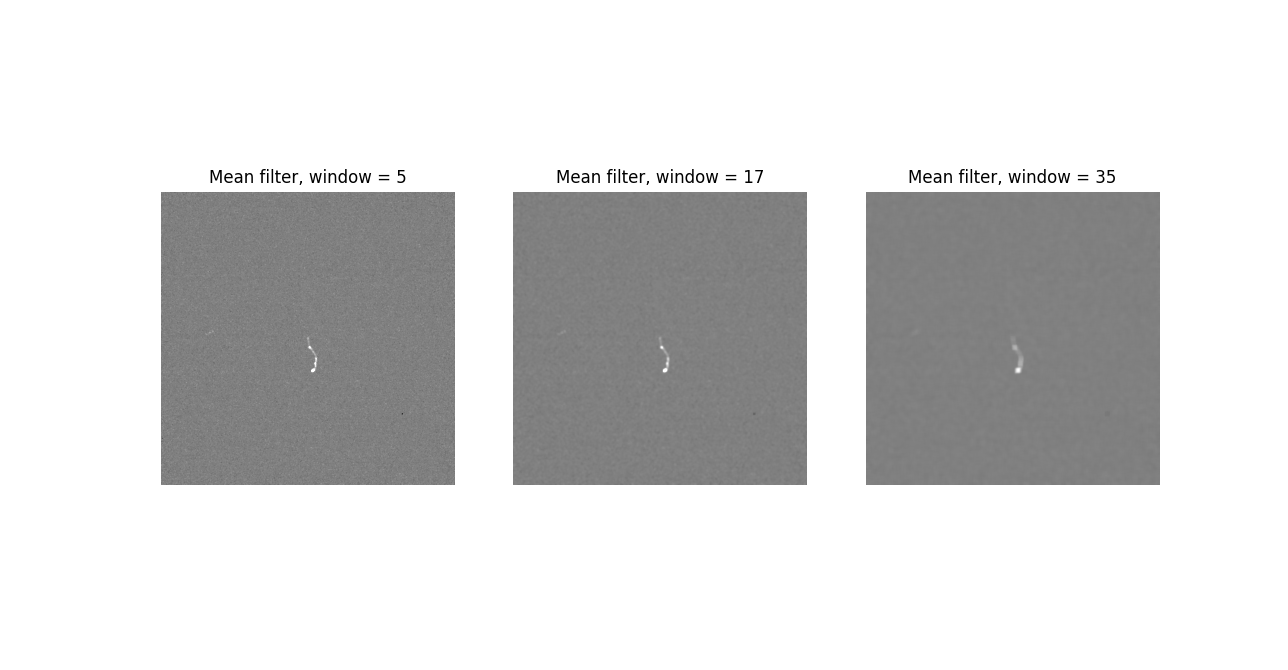
\includegraphics[width=1\textwidth]{image_files/mean_example.png}
\caption{Mean filtering process example}
\label{mean_example}
\end{figure}


\begin{figure}[H]
\centering
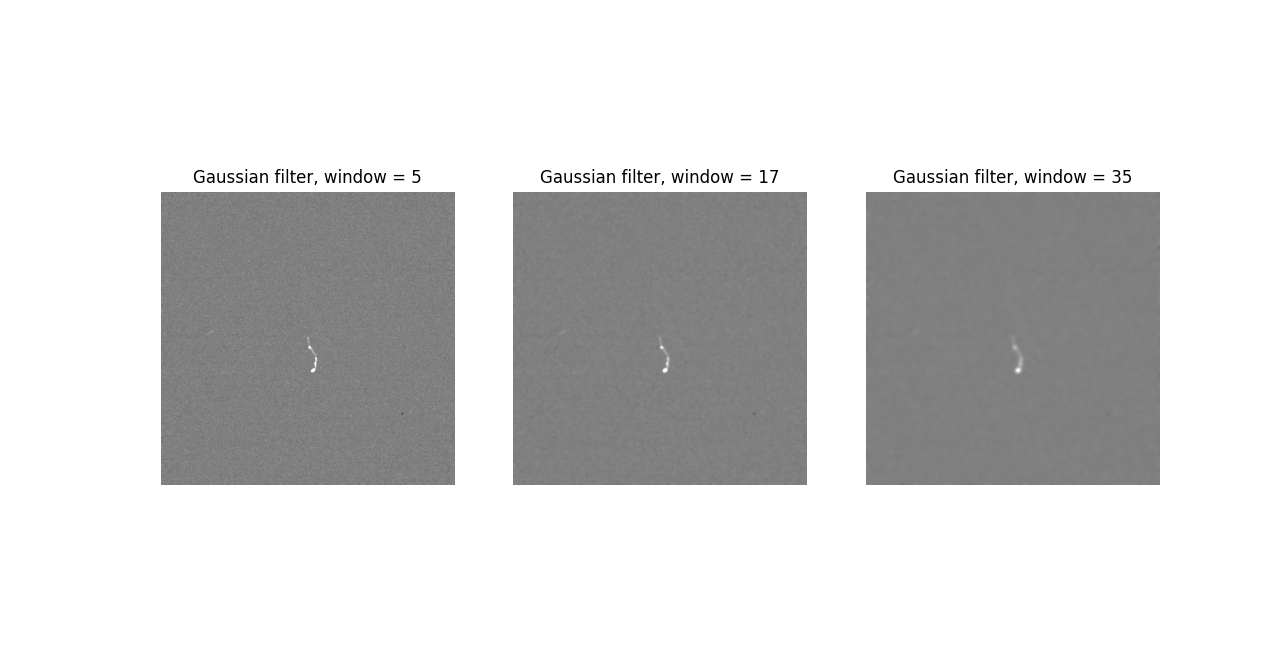
\includegraphics[width=1\textwidth]{image_files/gaussian_example.png}
\caption{Gaussian filtering process example}
\label{gaussian_example}
\end{figure}


\begin{figure}[H]
\centering
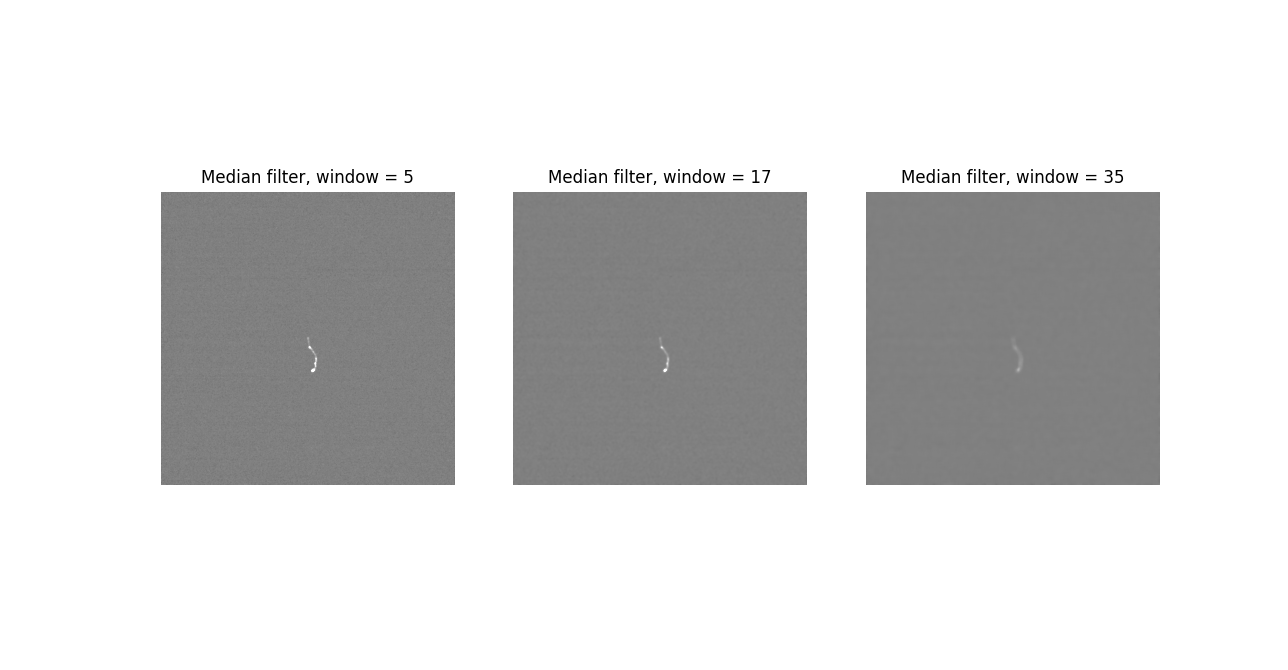
\includegraphics[width=1\textwidth]{image_files/median_example.png}
\caption{Median filtering process example}
\label{median_example}
\end{figure}




\subsubsection{Deep Learning based}
For a deep learning based, the U-Net %%\ref{} referenciar a revisao bibliografica%%
was used to perform a pixel selection task. The idea behind this usage is that each pixel returns a value between 0 and 1, which reflects the probability of a pixel being considered a signal pixel. The closer to 1, the more likely such a pixel is to be a signal. On the other hand, the closer to 0, the greater the chance that the pixel is background.

The U-Net implementation has been based on architechture proposed by \ref{ronneberger2015u}, by changing the input image size. As the images of experiment have a 2048x2048 size, the input layer and output layer of the neural network was changed from 572x572 to 2048x2048. The proposed network architecture is shown in appendix \textcolor{red}{referenciar apendice}. 

The figure \ref{unet_inou_example} shows a example of input that can be used for U-Net training along with an example of output presented to the neural network. All pixels that have their truth value greater than 0, are tagged as 1, otherwise are tagged by 0.

As the expected output of U-Net should be a probability of pixel be signal, the output layer that was chosen is Sigmoid that is 
commonly used for binary classification problems.


\begin{figure}[H]
\centering
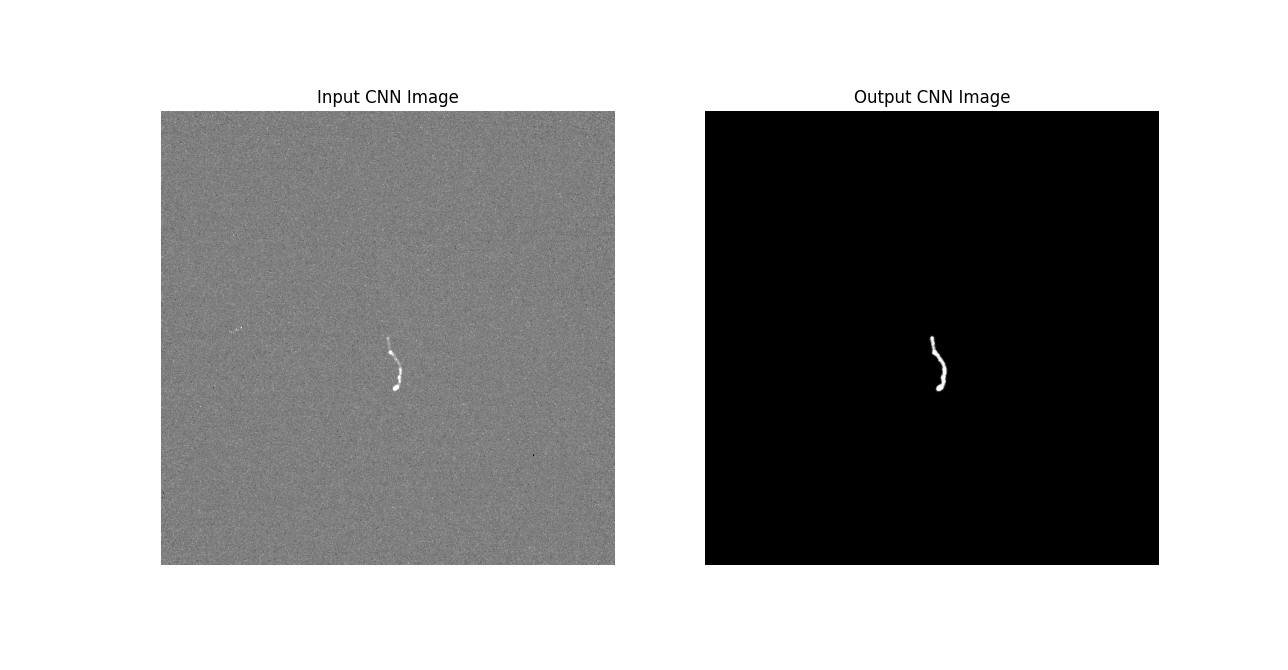
\includegraphics[width=1\textwidth]{image_files/cnn_input_image_example.png}
\caption{Input x output U-Net example}
\label{unet_inou_example}
\end{figure}

Once defined the architecture and the images that will be used for U-Net development, the next step is to train it. For the U-Net training to be feasible, it is necessary to know the ground truth of each image in order to present them to the neural network, minimizing the error function chosen, which in this case, the binary cross entropy was used , described by the equation \ref{cross_entropy}, where y is the truth pixel label and p is the probability returned by U-Net.

\begin{equation}
    L = -{(y\log(p) + (1 - y)\log(1 - p))}
\label{cross_entropy}
\end{equation}


A great need for solving problems involving deep learning is the demand for samples in the training process, especially in long tail problems, when there is little representation for some classes or dataset characteristics \ref{cui2019class}. As the simulation dataset has only 100 events for each particle type, at each energy level. A strategy was adopted was to create new samples, not using the original samples, leaving them for the U-Net evaluation stage. For this, a known process for this type of task was used, the data augmentation defined by \ref{shorten2019survey} as a data-space solution to the problem of limited data.



The main objective of data augmentation in the present work is to increase the sample size, without losing the main characteristics of the data used for training. In order to maintain such characteristics, such as format, energy of events and also of electronic noise, only rotation and translation transformations were used to generate new images. In order to do that, the equation \ref{da} was applied to original images pixel, for $x_{0}$ and $y_{0}$ translation parameters and $\theta$ the rotation parameter, in order to generate new images based on the original. It's importante to note that Data Augmentation process was applied before noise inserting, keeping noise characteristics for generated images. An example of $\theta$ = 25° rotation is shown in figure \ref{data_aug_example}.


\begin{equation}
 \begin{bmatrix} x' \\ y' \\ 1 \end{bmatrix}
 =
  \begin{bmatrix}
   cos(\theta) & -sen(\theta) & x_{0}\\
   sen(\theta) & cos(\theta) & y_{0}\\
   0           & 0           & 1 
   \end{bmatrix}
   \begin{bmatrix}
    x \\ y \\ 1
   \end{bmatrix}
   \label{da}
\end{equation}


\begin{figure}[H]
\centering
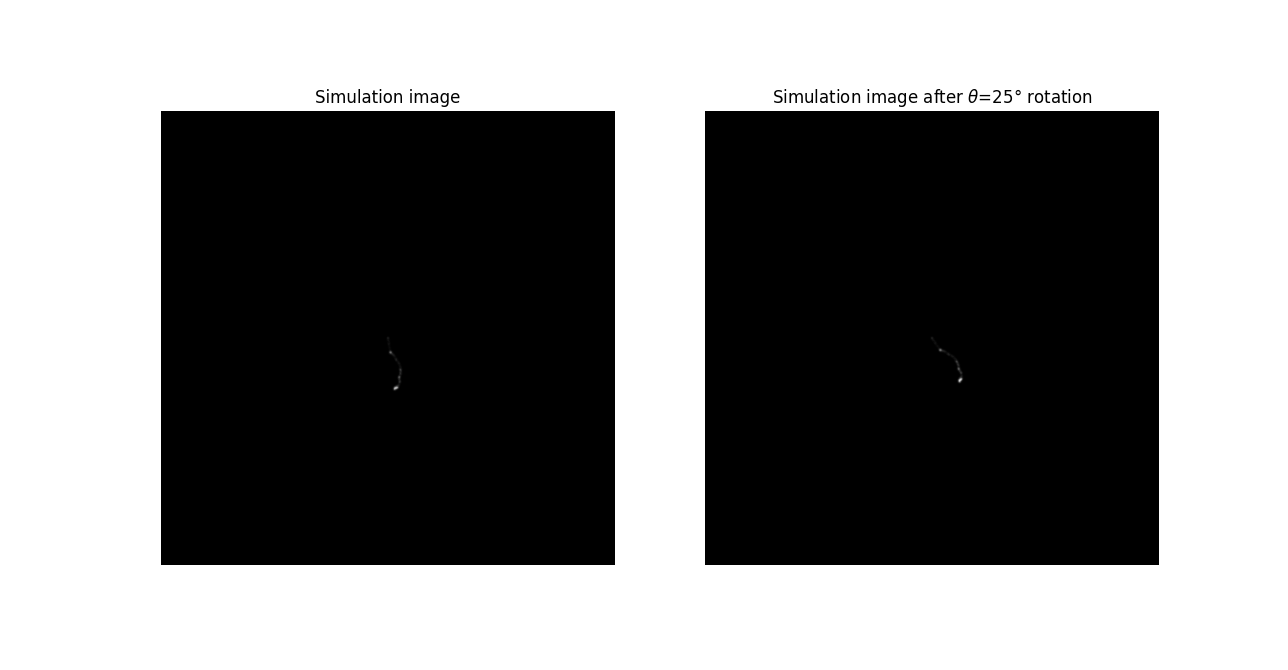
\includegraphics[width=1\textwidth]{image_files/data_aug_example.png}
\caption{Data augmentation example}
\label{data_aug_example}
\end{figure}


Based on the definitions made, the next step is to train the network to evaluate the results. With the data augmentation process, 10000 images were generated for training the neural network, of which 7000 (70\%) were used for training and 3000 (30\%) for validation. The network was trained for 50 epochs, with 450 steps per epoch at a learning rate of 0.02. The optimizer used for this task is Adam Optimizer \ref{defossez2020convergence}, since it normally presents a fast convergence in relation to the other. The figure \ref{train_unet} shows the training process for U-Net. 


\begin{figure}[H]
\centering
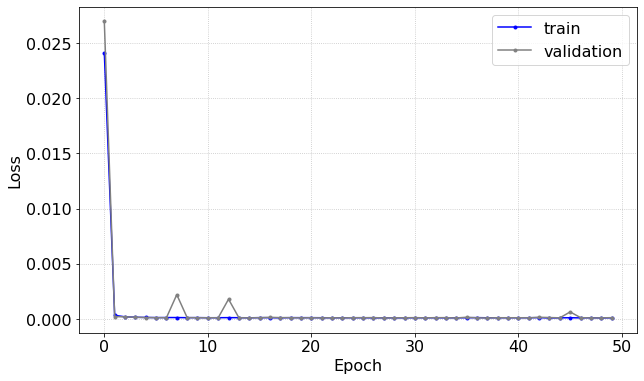
\includegraphics[width=1\textwidth]{image_files/u-net_train.png}
\caption{U-Net training process}
\label{train_unet}
\end{figure}

It's possible to notice that after few epochs, the loss function for training and validation data tends to a small value. In some epochs, the value o validation datasets presents some peaks. This can happens because some batch of images of validation can be more complex to predict (Low energy, for example), but this peaks appears to decrease along to training epochs.

Once filters and the U-Net, the next step is to define a metric to evaluate the efficiency of those algorithms. The chosen metrics are defined in the next section.

\subsection{Efficiency}

One of the most important steps of the reconstruction algorithm is the pixel selection step. The mainly goal of this step is to maximize the number of signal pixels that are signal in fact on the output and minimize the number of background pixels classified as signal by that step, also known by SNR (Signal noise ratio). 

There are several ways to measure how good a classifier is, which in this case can be considered as one, since an algorithm is being used to infer whether a certain element (pixels in this case) are part of a previously defined group. As each simulation image has only 1 event, the percentage of pixels filled in an image is extremely small, about 0.01\%. Some metrics as accuracy or ROC curve may lead us to think that the classifiers are performing well when in fact they are not, because it is a problem of unbalanced classes. Because of that, the metrics that was chosen at this step are commonly used for this kind of problem, Precision  and Recall \cite{juba2019precision}, that can be defined by equation \ref{eq10} and \ref{eq11}, respectively.


\begin{equation}
    Precision = \frac{TP}{TP+FP}
    \label{eq10}
\end{equation}

\begin{equation}
    Recall = \frac{TP}{TP+FN}
    \label{eq11}
\end{equation}

Where, TP are the signal pixels classified as signal pixels, FP are background pixels classified as signal pixels and FN is the signal pixels classified as background. Changing the threshold value, a Precision-Recall curve can be built, in other to evaluate all possible operation points, as shown on figure \ref{precision-recall-example}


\begin{figure}[H]
\centering
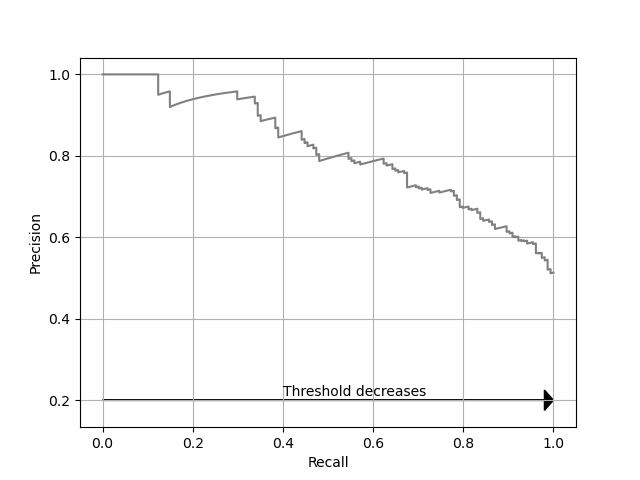
\includegraphics[width=0.7\textwidth]{image_files/precision-recall-example.png}
\caption{Precision-Recall curve example}
\label{precision-recall-example}
\end{figure}




Thinking about images and threshold, when using a high threshold, it means that most of the pixels that exceed this value have a high intensity value and are probably actually part of a cluster of some particle. In other words, most of the pixels classified as signal, in fact are implying a high value of precision. For recall, as the threshold value is high, most of the lower intensity pixels will be rejected by the threshold, presenting a lower value. 

Looking at it from the inverse perspective, when the threshold value is low, most of the pixels are classified as a signal, and therefore, probably most of the pixels that are actually a signal will be identified, generating a high recall value. On the other hand, a low threshold value generates a large volume of background pixels classified as a signal, thus causing a decrease in the precision value.


Each pair (filter, parameters) or any filter selection technique will have their own Precision-Recall curve, by changing threshold value and calculating Precision and Recall. Therefore, one way to choose the best parameter for a filter would be the best precision-recall curve. But how to choose the best curve? 

To perform this task in a systemic way, a summary measure of the precision-recall curve can be used, and for this work, the F1-score will used as can be defined by equation \ref{eq12}.

The F1-score is the harmonic mean of precision and recall \ref{flach2015precision} and is a metric that has a lower and an upper bound, that in this case are 0 and 1, respectively.


\begin{equation}
    F1 = \frac{2*Precision*Recall}{Precision+Recall} = \frac{2*TP}{2*TP+FP+FN}
    \label{eq12}
\end{equation}

Looking into equation \ref{eq12}, its possible to noticed that the maximum value of F1 score is when precision and recall are equals to 1. When precision or recall are zero, the F1-score also are.

Each pair precision and recall brings to one F1-score value. To summarize each precision-recall curve, the maximum value will be chosen and it will represent how efficient is a filter comparing with the ground truth.



\chapter{Results}
\label{chap:result}

%\section{Proposed method for performance measurement in the CYGNO environment}

As mentioned before, the main objective of this work is to verify if digital filters have the potential to produce relevant improvement of the signal-to-noise ratio of the events produces with the LEMOn detector.
In other to accomplish that, a set of measures should be defined and evaluated. On this work, the proposed evaluation is divided into 3 parts. (1) pixel selection performance; (2) assessment of the impact of filters on the reconstruction algorithm; and (3) real data analysis.
In addition to being used for performance comparison between filters, the results of step (1) will also be used to select the best filters parameters based on simulated images, as shown on figure Simulation environment. 
Once filters parameters are chosen, step (2) will evaluate their impact on the CYGNO reconstruction algorithm. The energy values provided by the simulation will be used to measure the filters' impact regarding energy estimation.
Finally, step (3) proposes a qualitative analysis based on energy histograms constructed from the output of the reconstruction algorithm and on the processing time spent by each of the proposed filters.
In all the steps, the version used by the CYGNO Experiment before insertion of the changes proposed in this work will also be compared.
All these steps will be presented in more detail in the next sections along with the achieved results.



Based on the proposed methodology and evaluation metrics for this step, we have a distribution of the best f1 score for each filter and parameter. The main goal of this step is to choose the best parameter for each filter based on best F1-Score distribution. By experimental results, for median, gaussian and mean, the window parameter was changed from 9 to 21. For U-Net, the parameters was got from training process. As the filter selection method of reconstruction algorithm use a simple cut based on the standard deviation of each pixel noise, none parameter should be used. In figures \label{f1median} \label{f1gaussian} \label{f1mean}, its possible to notice the value of the best F1-score for each filter parameter in all dataset, for each kind of particle. The best parameter will be chosen from maximum point of each filter curve, and those values are shown in table \ref{f1resume}.

\begin{figure}[H]
\centering
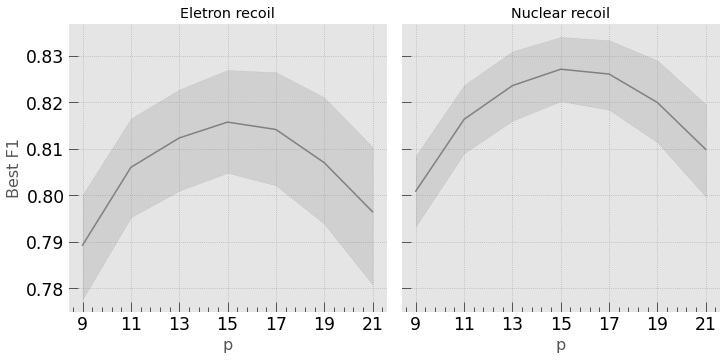
\includegraphics[width=0.7\textwidth]{image_files/median_f1.png}
\caption{F1-Score median parameters}
\label{f1median}
\end{figure}


\begin{figure}[H]
\centering
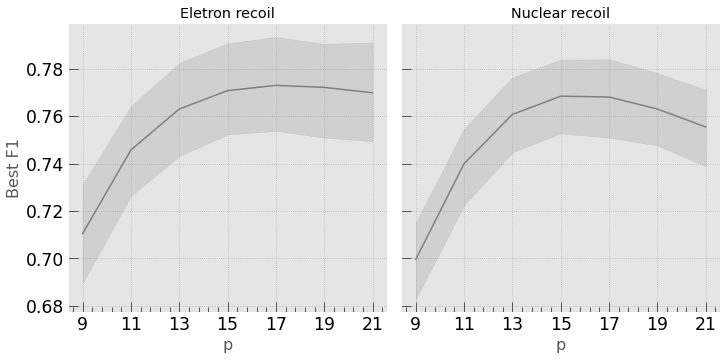
\includegraphics[width=0.7\textwidth]{image_files/gaussian_f1.png}
\caption{F1-Score gaussian parameters}
\label{f1gaussian}
\end{figure}

\begin{figure}[H]
\centering
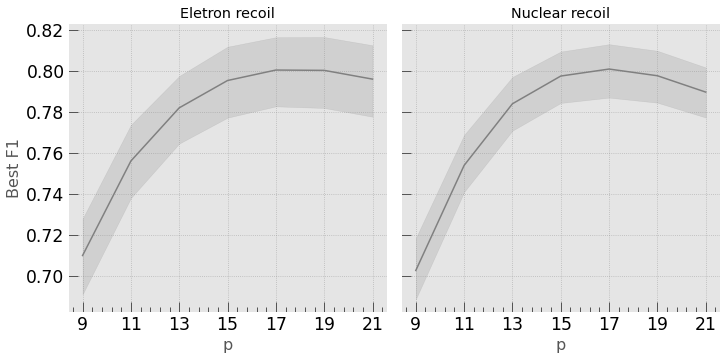
\includegraphics[width=0.7\textwidth]{image_files/mean_f1.png}
\caption{F1-Score mean parameters}
\label{f1mean}
\end{figure}


\begin{table}
\begin{tabularx}{0.8\textwidth} { 
  | >{\raggedright\arraybackslash}X 
  | >{\centering\arraybackslash}X 
  | >{\raggedleft\arraybackslash}X | }
 \hline
 Algorithm & Particle & Best F1 (\mu \pm \sigma) \\
 \hline
 Cygno   & Electron recoil &  0.172 \pm 0.157  \\
 \hline
 Cygno   & Nuclear recoil &  0.102 \pm 0.073  \\
 \hline
 U-Net   & Electron recoil &  0.873 \pm 0.083  \\
 \hline
 U-Net   & Nuclear recoil  & 0.874 \pm 0.040  \\
 \hline
 
\end{tabularx}
\label{f1resume}
\end{table}


It is possible to notice that the distribution of the best f1 scores for when the algorithm uses filtering processes present the best results, remembering that the maximum (and best) value of f1-score that it is possible to obtain is 1.
Another point of importance is regarding the variance of the best f1-scores. The variance of this value is due to the intensity value of the tracks in the image. Images where the track has low energy tend to have a lower F1-score when compared to higher energy tracks. This can also occur in the case of electron recoils, where there is great variation in intensity along the track in the images.
The best parameters for each filter can be choose by looking at the figures  \label{f1median} \label{f1gaussian} \label{f1mean} and the table for cygno and U-Net algorithms. For gaussian and mean the parameter (w) is 17 and for median, the window that was chosen is 15. A resume of this values and the respective descriptive statistics for best F1 score can be noticed on table bellow.


\begin{tabularx}{0.8\textwidth} { 
  | >{\raggedright\arraybackslash}X 
  | >{\centering\arraybackslash}X 
  | >{\raggedleft\arraybackslash}X | }
 \hline
 Algorithm & Parameter & Best F1 (\mu \pm \sigma) \\
 \hline
 Median   & 15 &  0.820 \pm 0.127  \\
 \hline
 Mean   & 17 &  0.800 \pm 0.184  \\
 \hline
 Gaussian   & 17 &  0.771 \pm 0.225  \\
 \hline
 Cygno   & None &  0.137 \pm 0.127  \\
 \hline
 U-Net   & Many  & 0.873 \pm 0.060  \\
 \hline
\end{tabularx}


Once the parameters chosen according to the established metric, the next step is to insert the filtering step in the entire reconstruction process and compare it with the current process in order to check if there were improvements. The CYGNO collaboration has developed a post-processing process, which aims to reduce the number of points sent to the clustering algorithm. This algorithm has a high computational cost and also uses a filtering process at this step. In order to assess the real gain in using filters, this algorithm will not be used when filters are applied to images.

The most important variable to measure at this step is the reconstructed energy at the output of algorithm. The mainly goal is to check if the algorithm proposed is able to reconstruct the input energy and compare it to reconstruction algorithm. Last but not least, the performance of the algorithms also will be evaluated and to do it, the processing time will be evaluated for all proposes at the same conditions.




% \begin{figure}[!htb]
% \centering
% 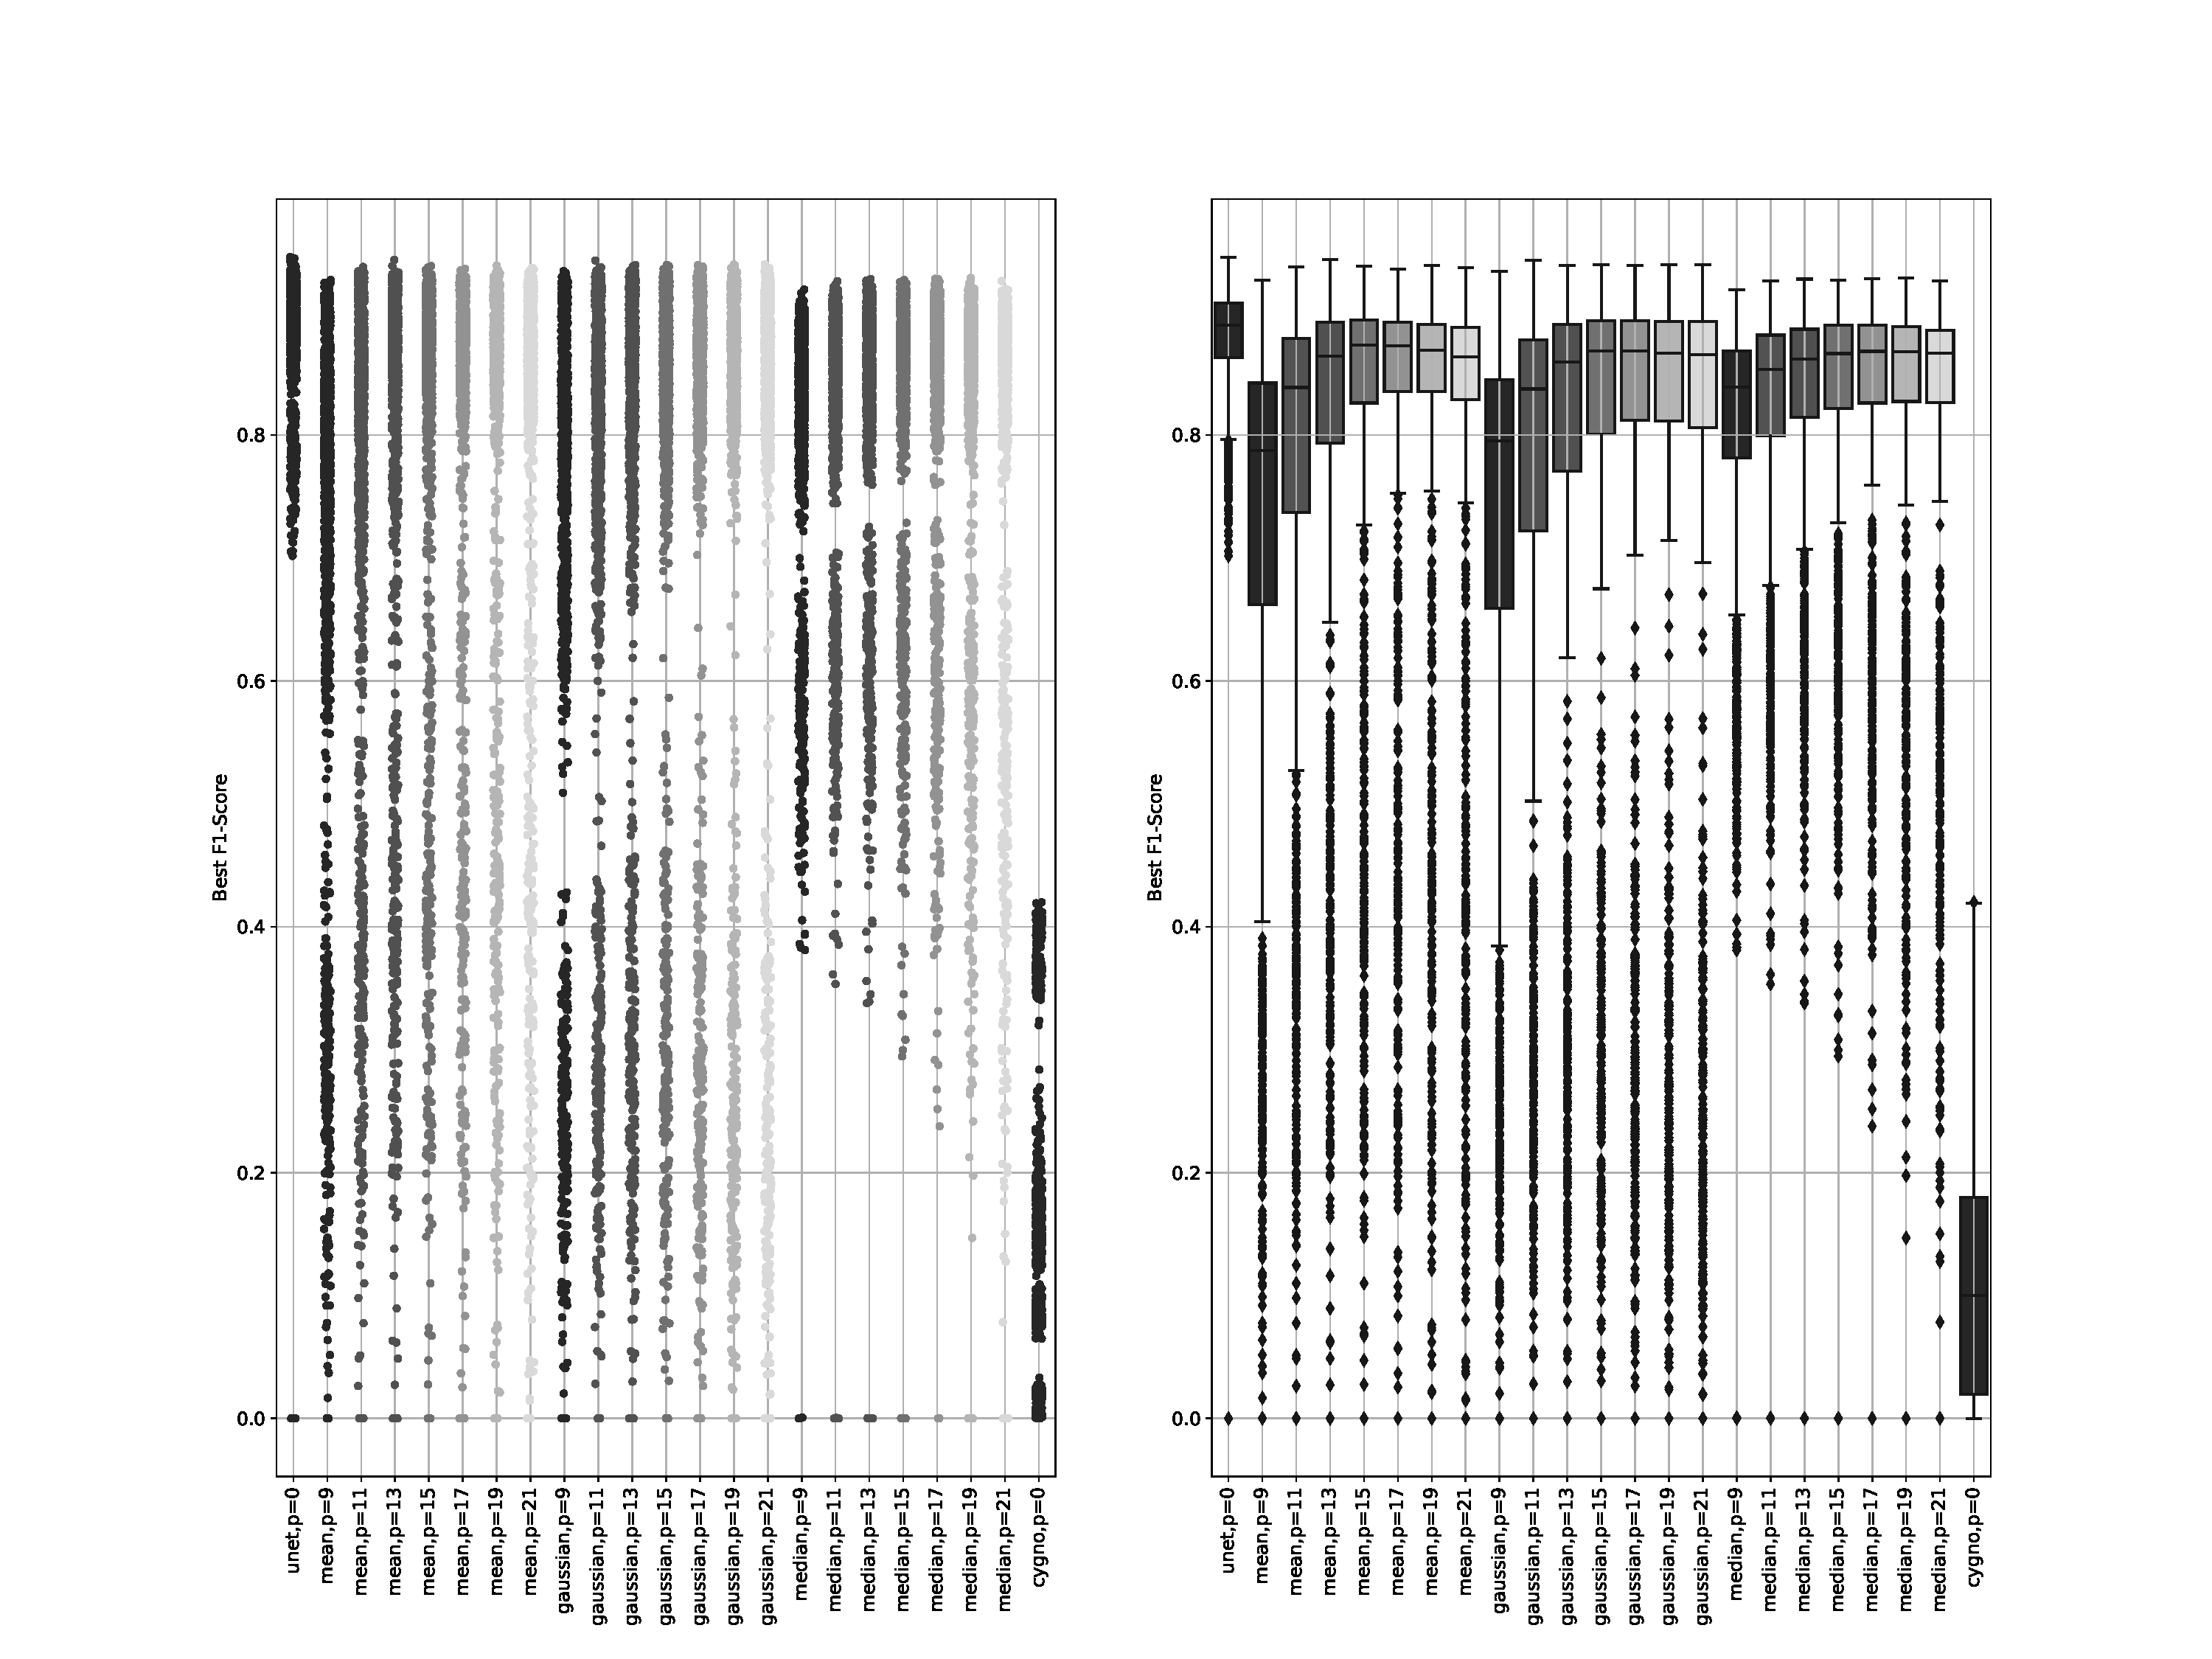
\includegraphics[width=0.5\textwidth]{image_files/f1_all.pdf}
% \caption{F1-Score filters}
% \label{f1score_all}
% \end{figure}


% \begin{figure}[!htb]
% \centering
% 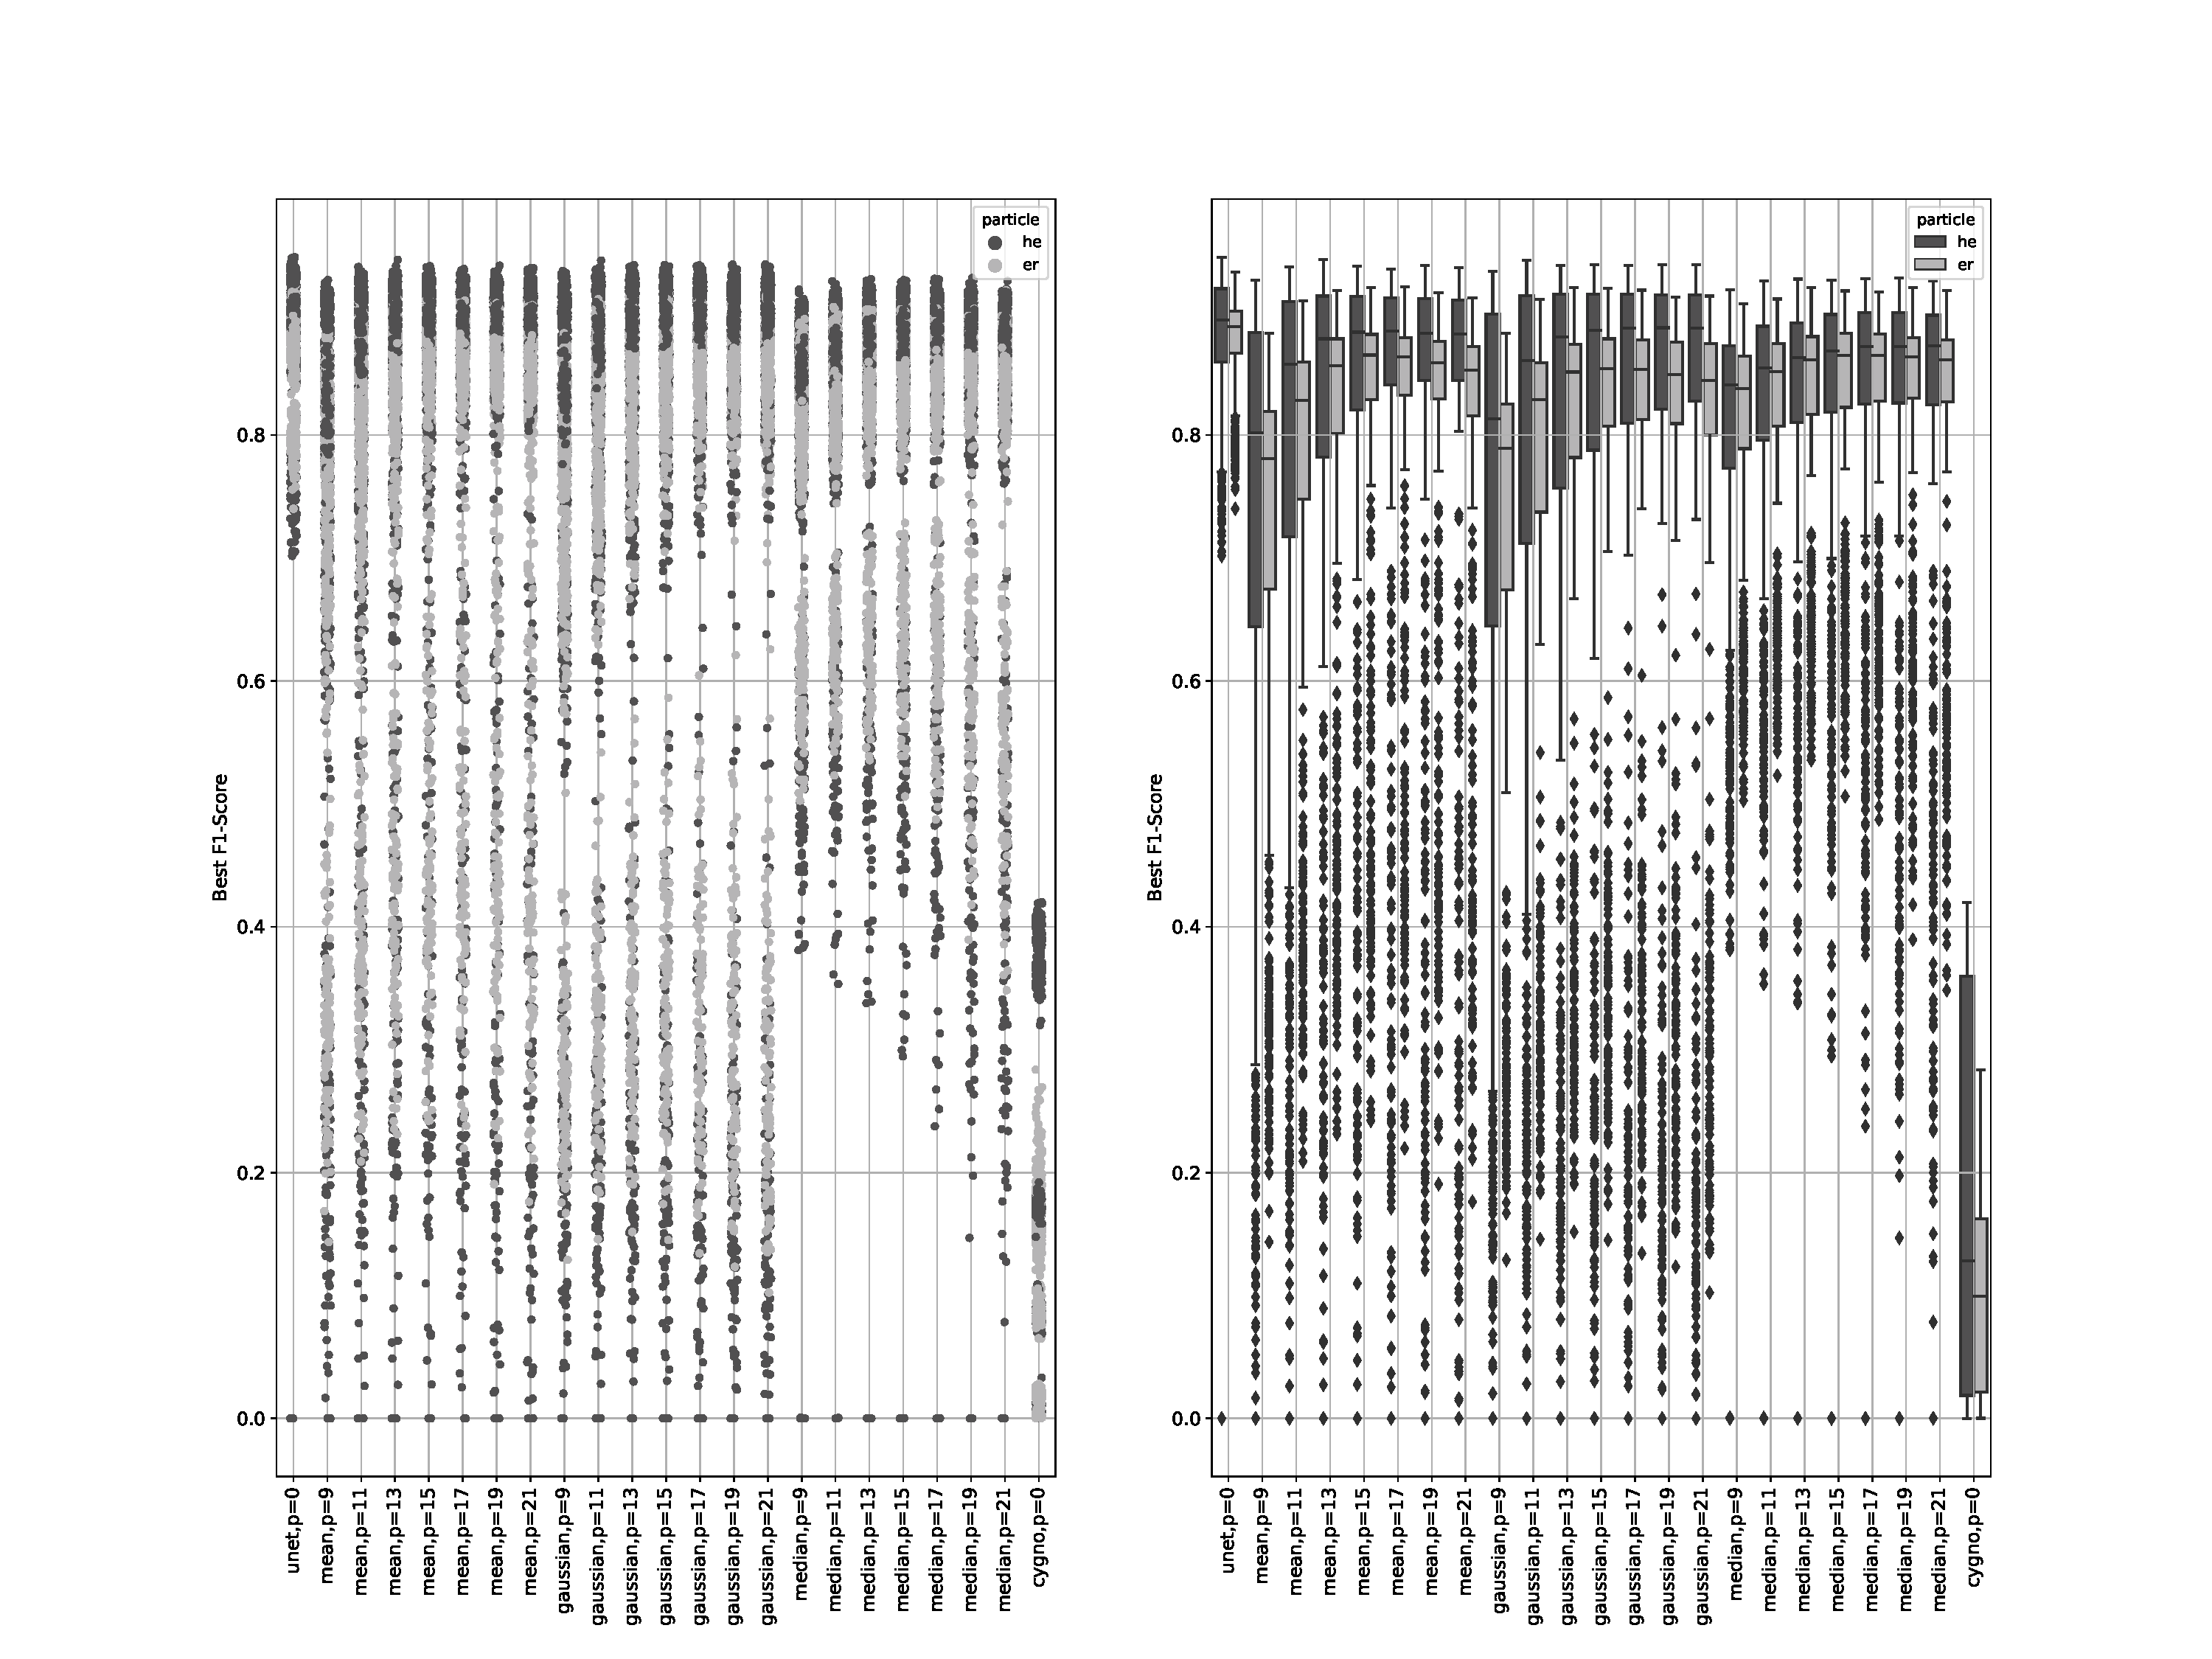
\includegraphics[width=0.5\textwidth]{image_files/f1_particle.pdf}
% \caption{F1-Score filters per particle}
% \label{f1score_particle}
% \end{figure}


% \begin{figure}[!htb]
% \centering
% 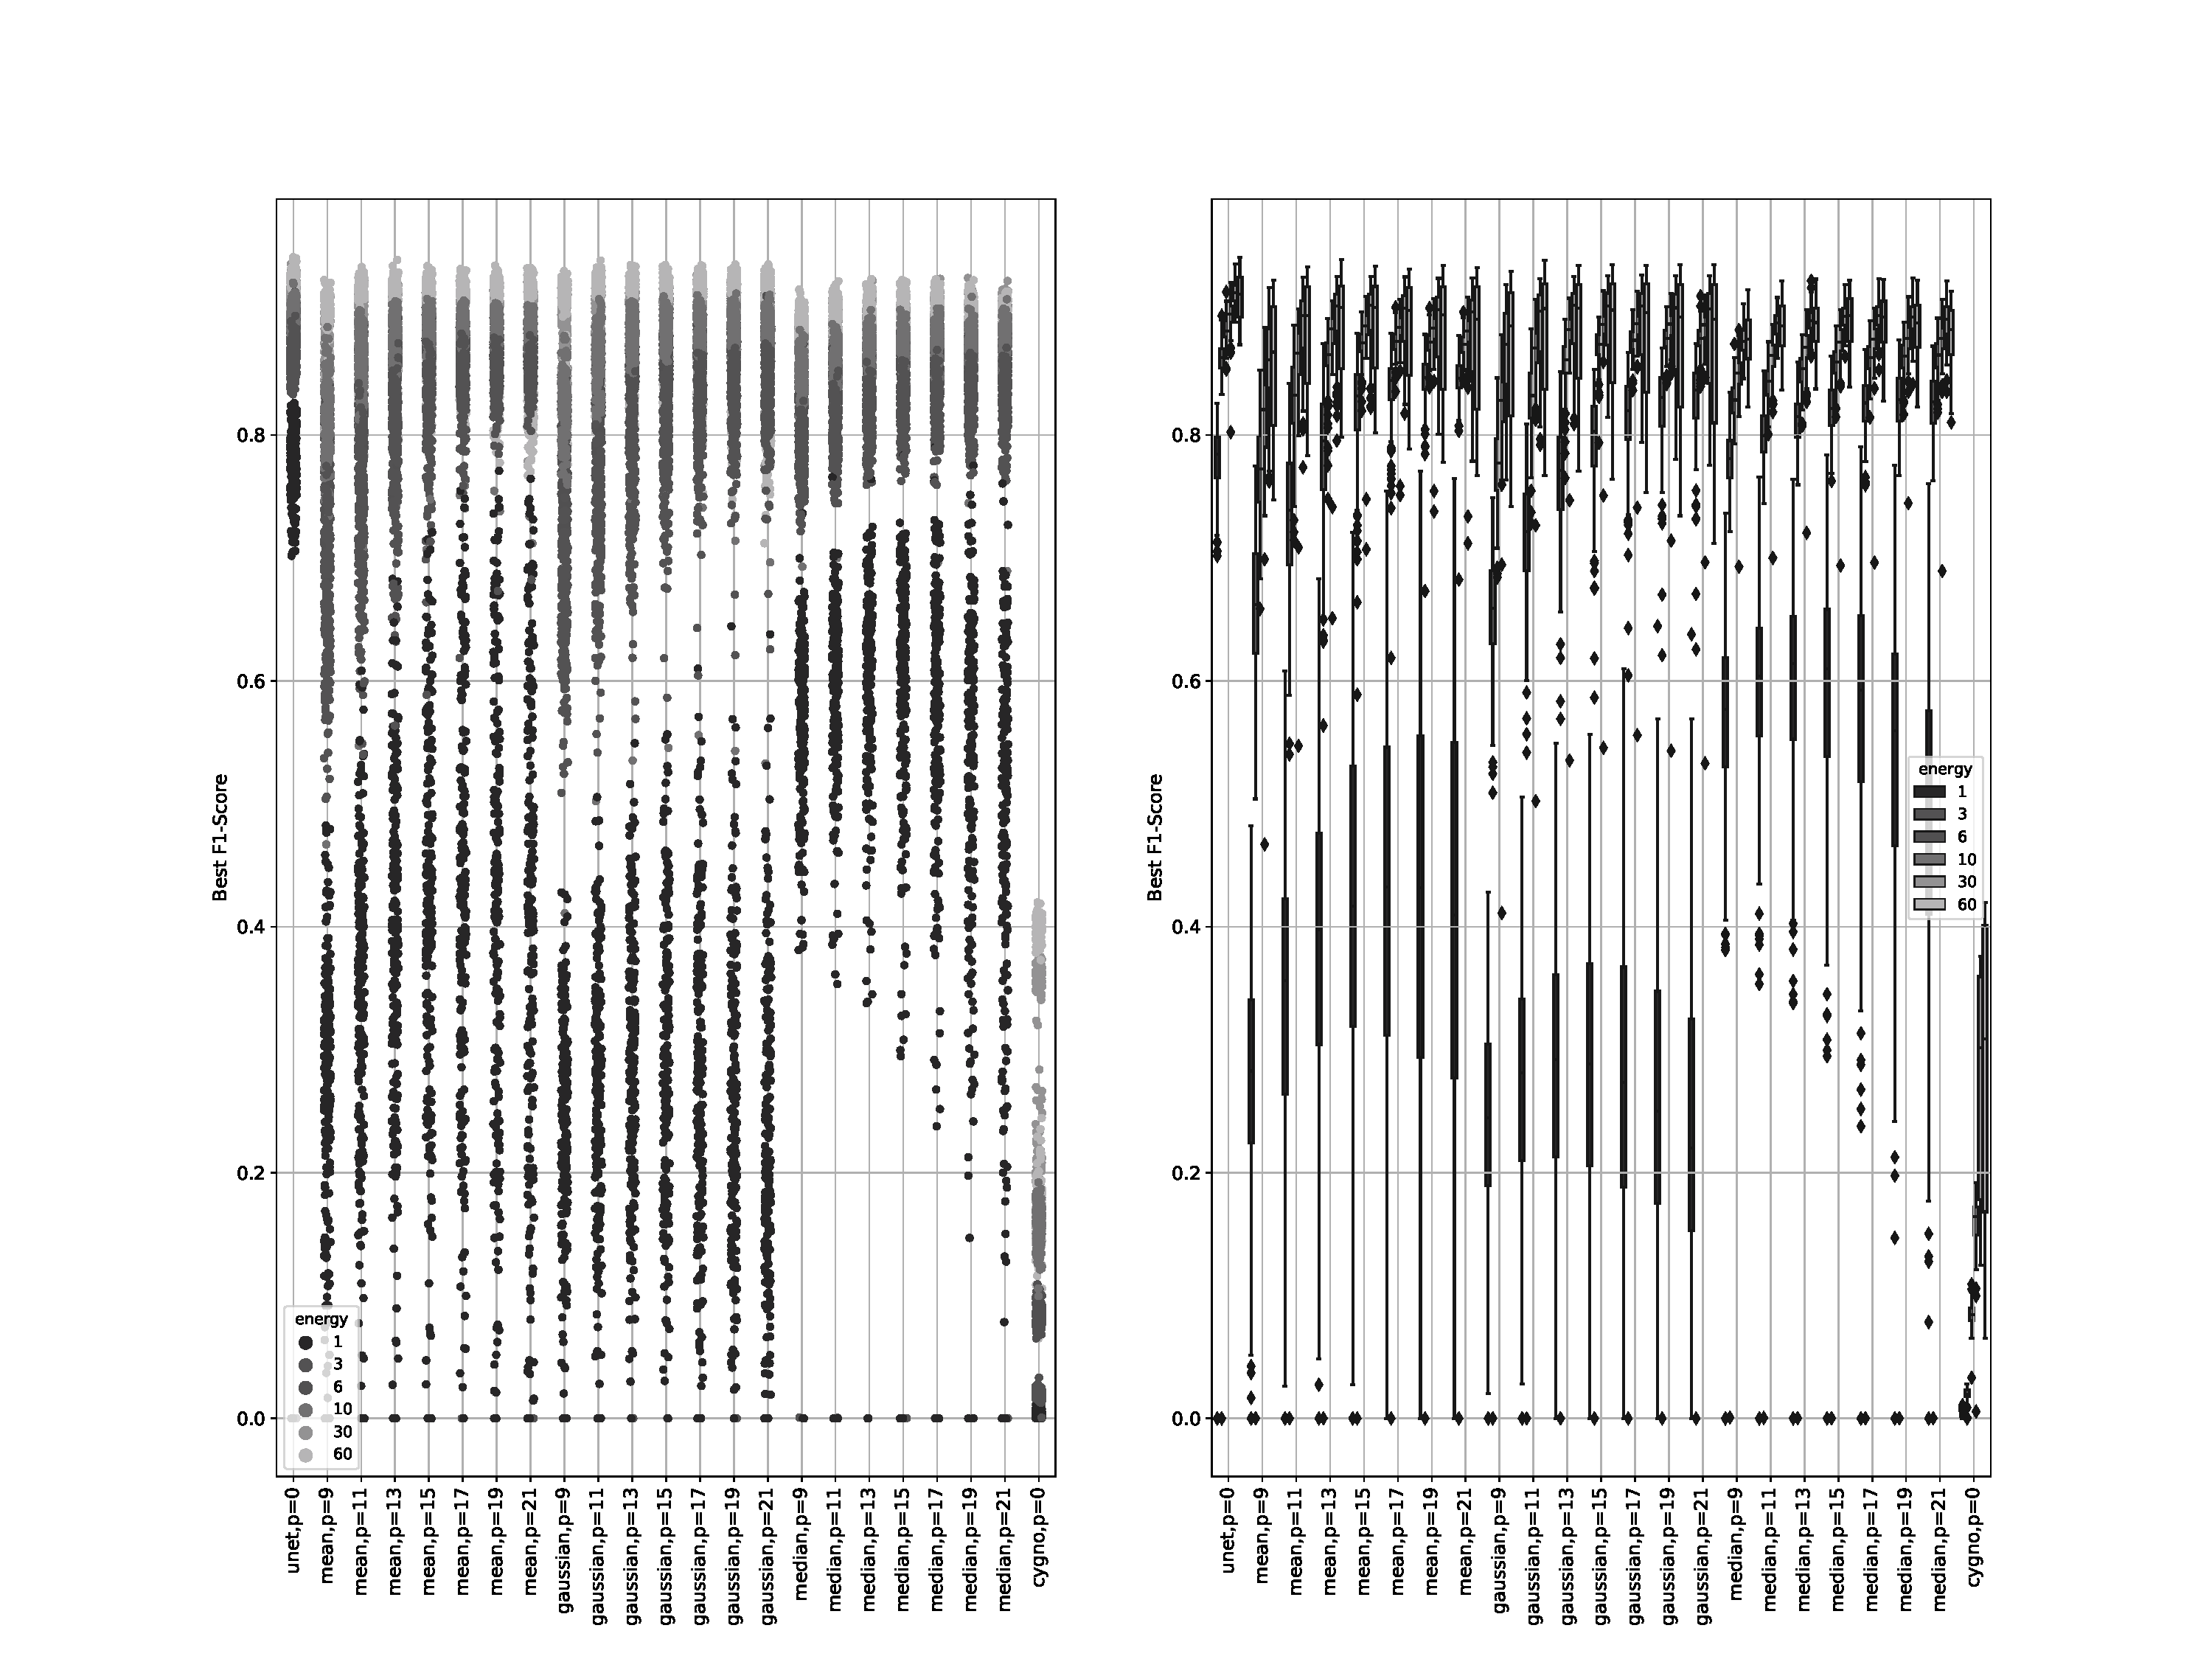
\includegraphics[width=0.5\textwidth]{image_files/f1_energy.pdf}
% \caption{F1-Score filters per image energy}
% \label{f1score_energy}
% \end{figure}


\section{Evaluating filters impact on reconstruction algorithm using simulation data}

If for choose the best filters and parameters at last step it was evaluate how efficient is some filter to select a pixel, now its necessary to measure how efficient is an algorithm to reconstruct some input feature, and for this case, energy will be this feature. The filters were treated similarly to a classifier where the output variable is categorical (is signal or not). Energy is a continuous variable and the approach more appropriate is dealing with it as a regression problem.

The simulation images has a characteristic that can be make this job simpler. Each simulation image has only one cluster, so is expected after clustering, one cluster and energy equal to energy at the input. A simple way to model it, is shown by equation \ref{eq13}, where $E_{o}$ is then output energy and $E_{i}$ is the input energy.

\begin{equation}
    E_{i} = \alpha E_{o} + \beta
    \label{eq13}
\end{equation}

At best scenario, each pair ($E_{o}$, $E_{i}$) will form a scatter plot and a linear model could be use to fit that points. In the ideal case, the intercept $\beta$ should be close to 0 and the slope $\alpha$ should be closer to 1. In this situation, the value of the reconstructed energy is the same of the input energy, but that alone is not enough. We can have these conditions met but with a linear model that does not fit the data. The quality of the linear fit also must be analyzed.

In order to do it, it will be measure two indicators that will evaluate the fit of the linear model to the data. The first, is the percentage of the variance of the data explained by the fit, that is known as $R^{2}$ and shown in equation \ref{eq14}, where $\sigma_{res}$ is the total variance of linear model and $\sigma_{tot}$ is the total variance of the data. When the total variance of linear model is small (good fit), $R^{2}$ value is closer to 1 but when it is closer to total variance of data (poor fit), $R^{2}$ value is closer to 0.

\begin{equation}
    R^{2} = 1 - \frac{\sigma_{res}}{\sigma_{tot}}
    \label{eq14}
\end{equation}

The $R^{2}$ is a important indicator of fit goodness but not only sufficient. This can be better explained by Anscombe’s quartet \ref{revell2018graphs}, that can be noticed in figure \ref{anscombe}.


\begin{figure}[!htb]
\centering
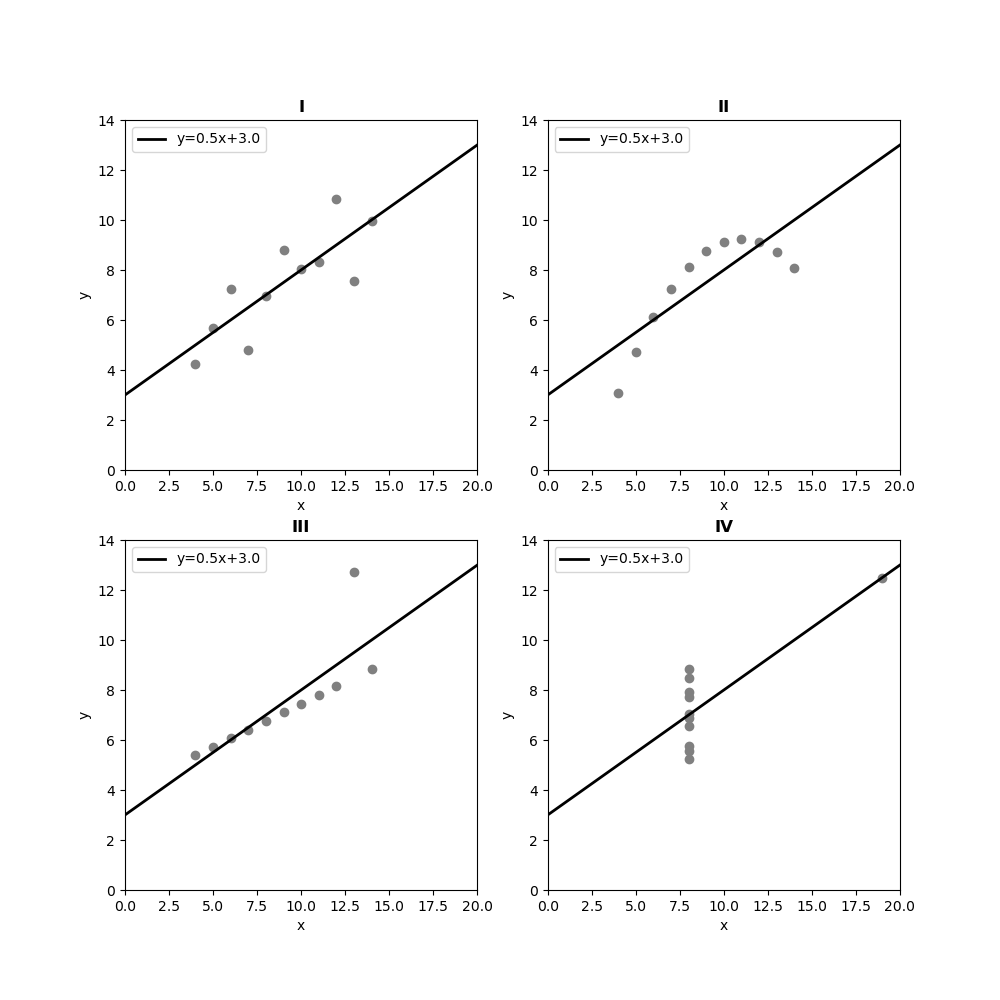
\includegraphics[width=0.7\textwidth]{image_files/anscombe.png}
\caption{Anscombe's quartet}
\label{anscombe}
\end{figure}

Its possible to see that all dataset are completely different but have the same mean, standard deviation and $R^{2}$. For adjustment purposes, just the first fit (I) is good, because there are a symmetrical behavior between the points and the linear fit. So for this work, a fit will be considered when the distribution of the error between the points of data and the fit follow a normal distribution. For validate this condition, a normality test will be applied to each fit.


As each dataset per energy and particle has 100 images, we will use the Shapiro-Wilk normality test \ref{razali2011power}, used for cases where the number of samples is reduced (less than 5000). For this test, the null hypothesis $H_{0}$ is that the tested distribution is not Gaussian, so when the $p-value$ of test is more than a threshold, the null hypothesis must be rejected and the tested distribution is Gaussian. The threshold value defined for reject or keep $H_{0}$ is 0.05 (5\%).

In the figure \ref{poor_fit_example}, it's possible to note the linear model is not fitted to the data. In addition to the low value of r squared, the error distribution between the points that make up the dataset is not Gaussian, as shown in the figure \ref{poor_fit_error_example}. The Shapiro-Wilk test was applied about the error and its possible to note that $p-value$ is closer to the 0.05, keeping the null hypothesis (Non Gaussian distribution).



\begin{figure}[!htb]
\centering
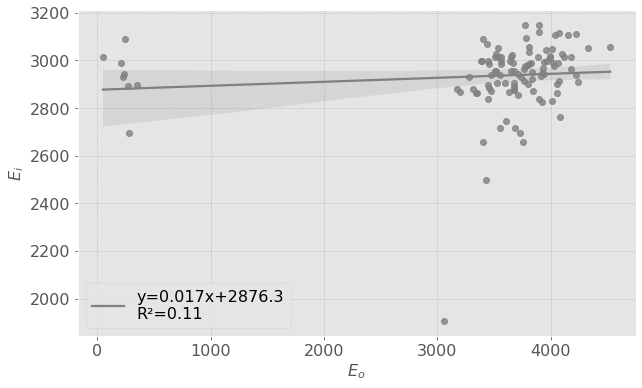
\includegraphics[width=0.7\textwidth]{image_files/fit_poor_ex.png}
\caption{Fit example}
\label{poor_fit_example}
\end{figure}


\begin{figure}[!htb]
\centering
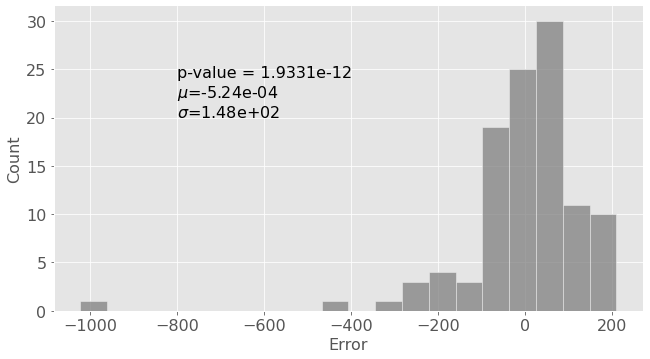
\includegraphics[width=0.7\textwidth]{image_files/error_fit_poor.png}
\caption{Error fit example}
\label{poor_fit_error_example}
\end{figure}


On the other hand, in the figure \ref{good_fit_example}, the linear model is a good approach about data distribution. The normality condition can be proven in figure \ref{good_error_fit_example}, where the error distribution is normal once p-value is greater than 0.05, rejecting the null hypothesis.


\begin{figure}[!htb]
\centering
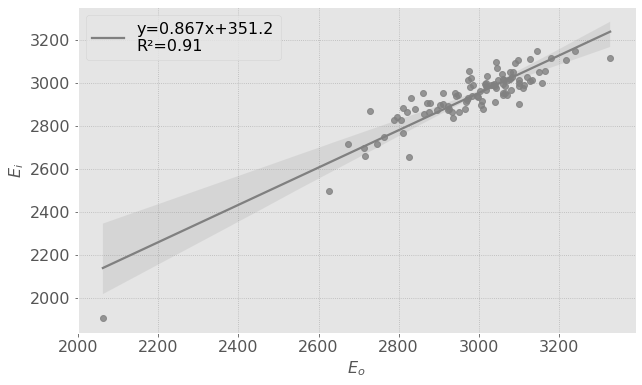
\includegraphics[width=0.7\textwidth]{image_files/fit_good_ex.png}
\caption{Fit example}
\label{good_fit_example}
\end{figure}


\begin{figure}[!htb]
\centering
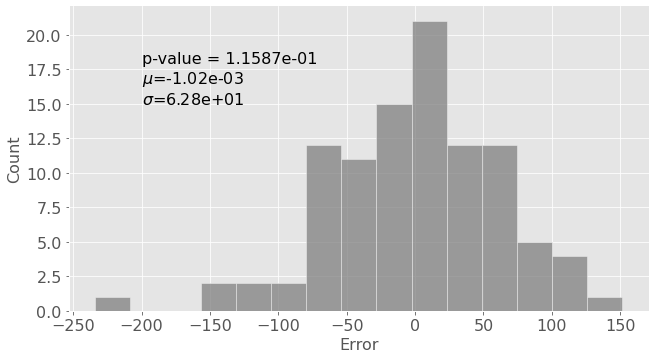
\includegraphics[width=0.7\textwidth]{image_files/error_fit_good.png}
\caption{Error fit example}
\label{good_error_fit_example}
\end{figure}

The metrics mentioned in this chapter will be the fomentation of the analysis that we will make of the reconstruction algorithm. The diagram in figure \ref{reco_diag} shows the evaluation methodology used to measure the performance of filters and the collaboration algorithm in the simulation images.

\begin{figure}[!htb]
\centering
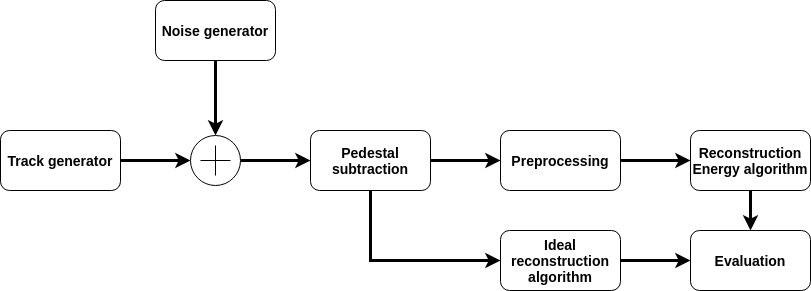
\includegraphics[width=0.7\textwidth]{image_files/reconstruct_diag.png}
\caption{Reconstruction algorithm evaluation flowchart diagram}
\label{reco_diag}
\end{figure}


The flowchart is similar the used to filters parameters evaluation and selection, but now the quantity evaluated is the energy. The reference for comparison will be a ideal clustering algorithm, where all signal pixels are identified and none background pixels belong to the formed cluster. The output energy of a ideal clustering algorithm can be obtained from the sum of intensities of all pixels. The intensity used for this analyse will the value of pixels after noise insertion and pedestal subtraction, because of the difficulty in rebuilding the original energy once altered by the noise insertion process .Then, the closer the proposed algorithm is to an ideal algorithm, the better it will be and we will use the metrics mentioned here to evaluate such performance. The threshold value also has been adapted, controlling this value to output a fix value of points after filtering, using a simple optimization algorithm. The advantage of this approach, is that also can used for real images and brings with it the idea of precision and recall, since many points after the threshold (low value) lead to a low precision value and few points (high threshold value) lead to a low recall value. A limitation is that it is based on the premise that each image has only one cluster, for the mapping of energies. For cases where this does not happen, a more elaborate analysis becomes necessary. Another assumption is about the shape of the clusters in the image. For particles, such as high-energy electron recoil (>=30keV), the tracks are no longer punctual, and instead have a curved shape, due to particle interactions in the detector. Often, such events are segmented by the clustering algorithm, making this type of analysis more complex. Therefore we consider nuclear recoils of 1, 3, 6 , 30 and 60keV, along with electron recoils of 1, 3 and 6keV for this analysis. Based on this, we selected the best results for each algorithm, based on the values of $R^{2}$, the number of clusters found and the guarantee of normality in the error distribution.


In the figure \label{r_square_result}, the value of $R^{2}$ is shown for each filter, energy and particle. Its possible to note that the value of $R^{2}$ begin low for low energy values for both proposes, but when U-Net or median filter are used, the value of that metric starts with good values. When energy value of particles increases, the value of $R^{2}$ also increases, reaching values close to the best case (1), except for collaboration algorithm.



\begin{figure}[!htb]
\centering
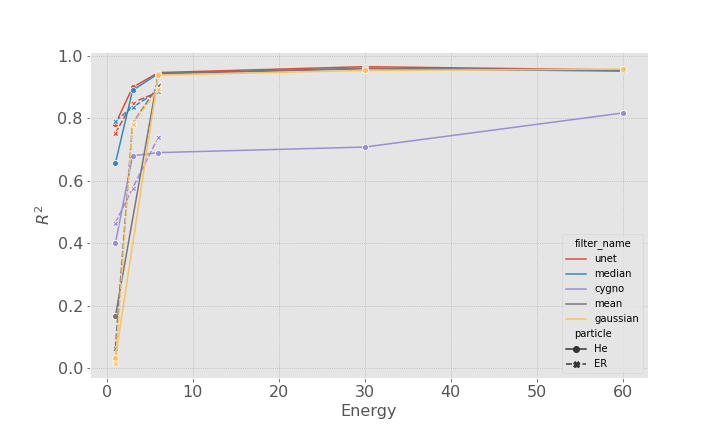
\includegraphics[width=0.7\textwidth]{image_files/r_square_result_sim.png}
\caption{R-squared evaluation}
\label{r_square_result}
\end{figure}

Looking into linear model parameters, in the figures \label{} and \label{}, its possible to notice the slope value and intercept of fittings, respectively. As the bias is not immune to scale, the value of bias was divided by the expected energy, for each case. This new value was called normalized bias ($\beta_{st}$). It's possible to see that U-Net and median shows good results as seen in $R^{2}$ analysis, once the ideal value of $\alpha$ is 1 and 0 for bias.



\begin{figure}[!htb]
\centering
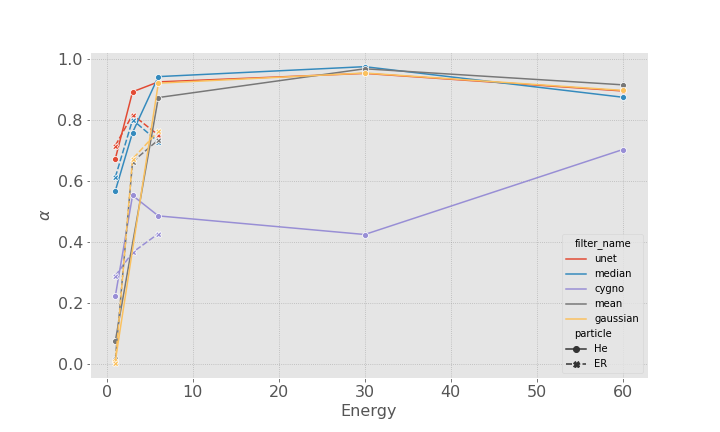
\includegraphics[width=0.7\textwidth]{image_files/slope_result_sim.png}
\caption{Slope evaluation}
\label{slope_result}
\end{figure}


\begin{figure}[!htb]
\centering
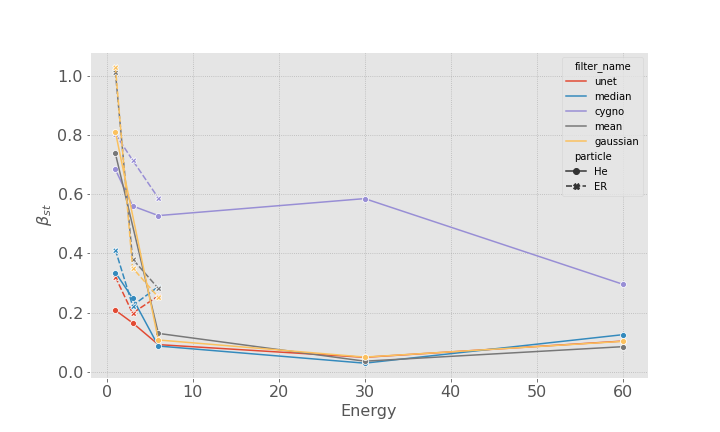
\includegraphics[width=0.7\textwidth]{image_files/beta_result_sim.png}
\caption{Intercept evaluation}
\label{intercept_result}
\end{figure}


Another important metric is the number of found clusters. Once the reconstruction energy shows interesting results, is necessary evaluate the identification clusters efficiency, since the reconstructed energy has already been evaluated. The figure \label{clusters_result} shows the percentage of clusters find in all image of energy packages. Not all filters can identify clusters in all images, but with increasing energy, this task becomes simpler, and the percentage of identified clusters increases considerably. Again, u-net and median were able to identify most of the clusters for all energy levels addressed in the analysis.



\begin{figure}[!htb]
\centering
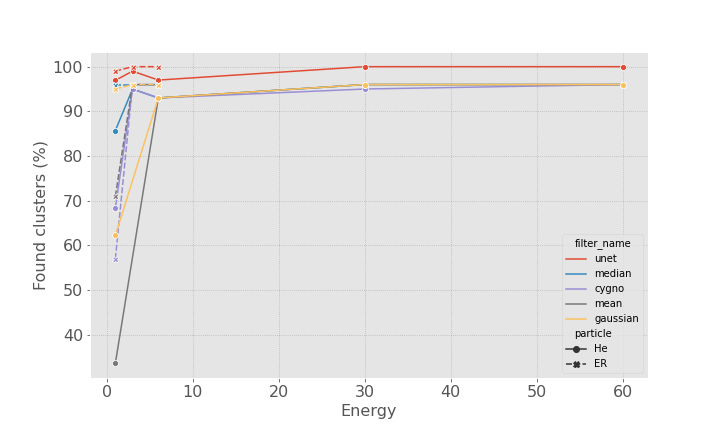
\includegraphics[width=0.7\textwidth]{image_files/clusters_result_sim.png}
\caption{Found clusters evaluation}
\label{clusters_result}
\end{figure}


\textcolor{red}{Falta uma conclusão para essa análise, abordando o ganho da utilização dos filtros nas imagens de simulação e preparando a análise nas imagens reais}






\section{Real results: Evaluating filters on reconstruction algorithm using real data}

After the methodology developed to evaluate the reconstruction algorithm and the proposed algorithm, using filters, in the simulation images, the next step consists in the validation of such methodology using real data obtained in the experiment. At this step, the filters that got the better results at simulation step (median and U-Net) were chosen to be evaluated on real data, the current colaboration algorithm also will be evaluated. An important point is that the same methodology cannot be applied, since we do not have a priori knowledge about the expected output, and therefore, there is no reference for comparing the result. What we will do is take advantage of part of the proposed methodology and qualitatively analyze some outputs of the reconstruction algorithm, for the output images of the detector.

This analysis will be divided into two parts, the first consists of evaluating the histogram of the reconstructed energy, aiming to compare with the output of the base collaboration algorithm. Another point that will be brought up in this analysis is the average processing time of the algorithm.

\subsection{Dataset}


\subsection{Reconstructed Energy}

As the main goal of this step is check the filters impact on reconstruction algorithm, the output energy when filters are used will be compared with the current algorithm used by collaboration. As the worked dataset has around 900 images, the reconstruction process for each one is time consuming, and therefore a very complex analysis, analyzing each operating point becomes unfeasible and therefore, we analyzed only 4 threshold values, 10000, 30000, 100000, 30000 points after threshold step. It's important to note that 300000 after threshold step is equivalent to $1.3\sigma$ threshold value, when collaboration algorithm is used. That is the threshold value used by experiment at threshold step.

In the figures \ref{median_real} and \ref{unet_real}, it's possible to see a comparison between the output energy distribution for each value of threshold that was defined, comparing the algorithm when median filter was used versus collaboration algorithm and U-Net versus collaboration algorithm, respectively.


\begin{figure}[!htb]
\centering
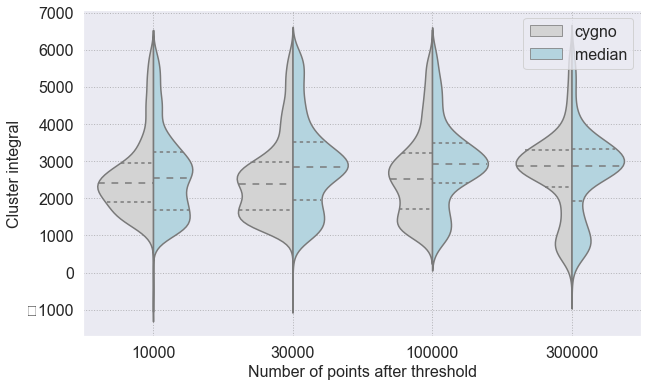
\includegraphics[width=0.7\textwidth]{image_files/real_median_cygno.png}
\caption{Median filter comparison}
\label{median_real}
\end{figure}


\begin{figure}[!htb]
\centering
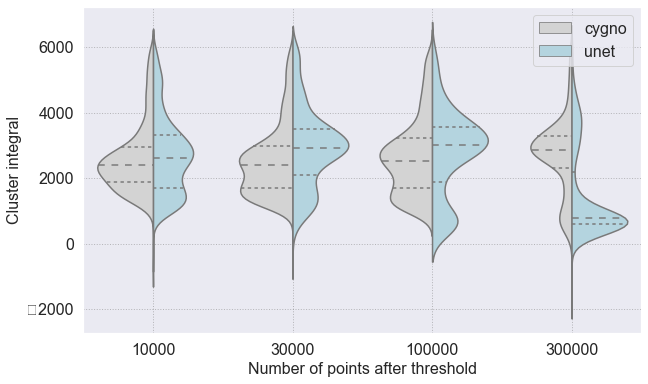
\includegraphics[width=0.7\textwidth]{image_files/real_unet_cygno.png}
\caption{U-Net filter comparison}
\label{unet_real}
\end{figure}


Looking into histograms, it is possible to notice that in the absence of filters, even with the post-processing algorithm, the collaboration algorithm does not present good results when the number of points after the threshold is small, since we have a high density of points in the low energy regions ( below 3000). This large volume comes from segmenting larger tracks into smaller, lower energy clusters. 

The median filter also presents the same behavior, but it indicates that the distribution starts to improve for lower point values after the threshold. In addition, with 300000 points after the threshold, the median filter presents an energy distribution very similar to the algorithm used by the collaboration, both in shape and in its descriptive measures.

For U-Net, a similar behavior can be seen, but at 300000 points after the threshold, the density of low energy values is very high, in relation to the other algorithms. The reason for this is the formation of low energy clusters due to the large volume of background events sent to the clustering algorithm.


To simplify comparisons, figures \label{median_real_keep} and \label{unet_real_keep} show a comparison very similar to the previous one, but now the collaboration algorithm always presents the same number of points after threshold (300000), which in this case would be the best scenario for such. 






\begin{figure}[!htb]
\centering
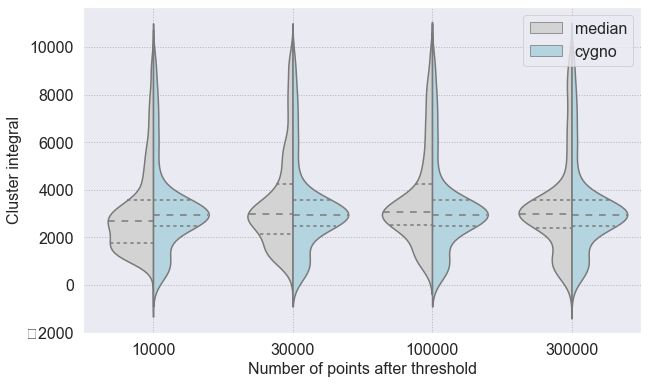
\includegraphics[width=0.7\textwidth]{image_files/real_median_cygno_keep.png}
\caption{Median filter comparison keep threshold for collaboration algorithm}
\label{median_real_keep}
\end{figure}


\begin{figure}[!htb]
\centering
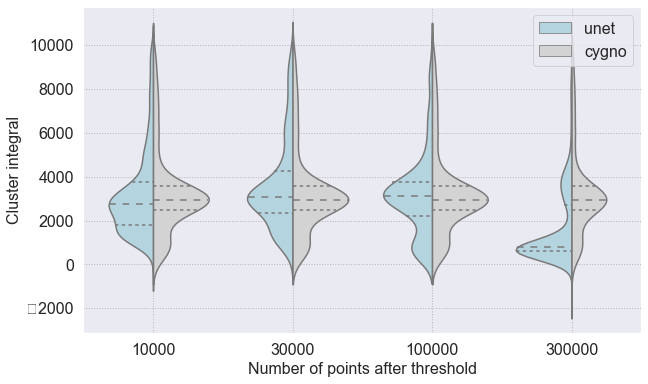
\includegraphics[width=0.7\textwidth]{image_files/real_unet_cygno_keep.png}
\caption{U-Net filter comparison keep threshold for collaboration algorithm}
\label{unet_real_keep}
\end{figure}

It is possible to see that with the increase in the number of points, the algorithm, when using the median filter, adjusts to the result obtained with the collaboration algorithm, and a complete adjustment takes place around 300,000 points. When using the U-Net, with the points defined in the analysis, it is not possible to obtain a perfect fit, however, the best scenario occurs much earlier, around 100000 points.


Based on the results obtained, it was visually noticed a great similarity between the energy distributions for the proposed configuration, when using a median filter and the configuration used by the collaboration algorithm, since in addition to the format, the descriptive measures of the distributions are very similar, as shown in the table below. In the figure \label{median_cygno_final}, it's possible to note the histogram of two energy reconstruction distribution, for Fe$^{55}$ region. The distributions appear to be very similar and it can also be noticed from descriptive statistics of the distributions, shown in table \ref{final_resume}. An important detail is that for the median filter, the value of the first quantile occurs at a lower energy value. This implies that such a configuration has a higher percentage of elements at higher energies. This may imply cluster union, which when using the collaboration algorithm, are partitioned into lower energy clusters. For the other quantiles, the statistics present approximate values.



\begin{figure}[!htb]
\centering
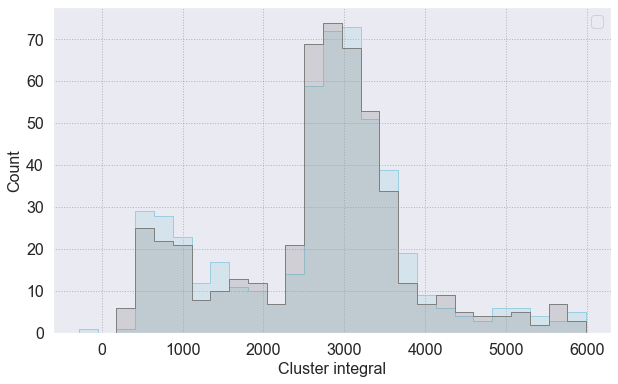
\includegraphics[width=0.7\textwidth]{image_files/final_compare.png}
\caption{Median x Cygno histogram comparision}
\label{median_cygno_final}
\end{figure}

\begin{tabular}{lrrr}
\toprule
\centering
{} &          $Q_{1}$ &          $Q_{2}$ &          $Q_{3}$ \\
filter\_name &              &              &              \\
\midrule
cygno       &  2298.399170 &  2857.923828 &  3291.806396 \\
median      &  1932.650269 &  2872.450195 &  3328.615234 \\
\bottomrule
\label{final_resume}
\end{tabular}


In order to statistically confirm whether the two distributions are the same, the Kolmogorov-Smirnov test \ref{berger2014kolmogorov} was applied about two distributions, to check if they are come from the same distribution. 

For KS test, the null hypothesis is that the distributions do not are from the same distribution, so if $p-value$ is greater than 0.05, the null hypothesis is rejected and the distributions come from the same distribution. The result for KS test about reconstructed energy distributions are shown in table \ref{ks}. As the p-value is greater than 0.05, the null hypothesis is rejected and the distributions of energy come from the same.


\begin{tabular}{rr}
\toprule
       KS &   p-value \\
\midrule
 0.050532 &  0.514255 \\
\bottomrule
\label{ks}
\end{tabular}

\subsubsection{Processing time}

From the analysis of the reconstructed energy, it was possible to perceive that the proposed algorithm can, at least, reproduce the same result, for output energy, when compared to the algorithm used by the collaboration. An important point in the analysis of this work is to verify the computational performance of such alteration, thinking in terms of the execution time of the algorithm. For the evaluation of this step, in each processed image, the processing time was calculated from the beginning of the pre-processing to the step of calculating the reconstructed energy. 

How to measure the processing time is a complicated task in terms of computation, since other processes may be running, interfering with the measurement of this quantity, to try to mitigate this effect, all algorithms were executed using cloud computing, ensuring that only such processes were running at the time of measurement.


In the figure \ref{total_time} shows the processing time boxplot for all evaluated scenarios, varying the number of points after the threshold. It's possible to see that for filters, median presents a high value when compared to U-Net. This happens because for U-Net, a GPU was used to image inference, reducing the time to perform the filtering. For collaboration algorithm, the processing time starts with a low value, but when the number of points after the threshold is high, this value increases considerably, being much higher than the others.

\begin{figure}[!htb]
\centering
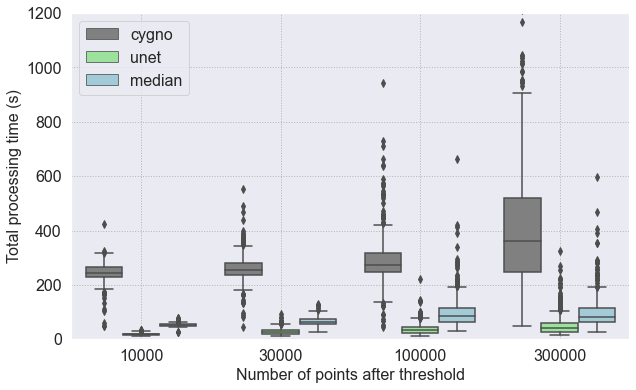
\includegraphics[width=0.7\textwidth]{image_files/time_total.png}
\caption{Processing time (All steps)}
\label{total_time}
\end{figure}


Perhaps such a procedure can lead us to think that the processing time should be the same, or very close for everyone when the number of points after the threshold is the same, but in fact this is not what happens. figure \ref{clustering_time} shows the clustering time for each evaluated scenario, between filters and number of post-threshold points. What can be seen, in the example where the number of after the threshold is large, the processing time is much longer, especially in the collaboration algorithm. This happens mainly because the dbscan is too sensitive to the number of points, and for this reason, rebinding is done, for example, since it reduces the number of pixels processed, and therefore, the computational complexity, which can reach $10^{4}$ times less \label{baracchini2020density}.
 
\begin{figure}[!htb]
\centering
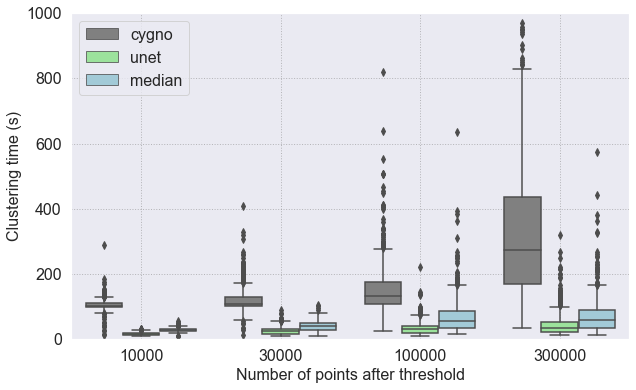
\includegraphics[width=0.7\textwidth]{image_files/time_clustering.png}
\caption{Processing time (Clustering step)}
\label{clustering_time}
\end{figure}


To confirm this hypothesis, figure \ref{rebin_eval} shows the relationship between the number of points after the threshold, and the number of points after the rebinding process, since these points are sent to the clustering algorithm, except for the collaboration algorithm, which has an additional noise removal step. It is possible to notice that the number of points after the rebinding process, for the collaboration algorithm is much higher compared to the filters, generating a longer processing time on the part of the noise reducer and the clustering itself.

\begin{figure}[!htb]
\centering
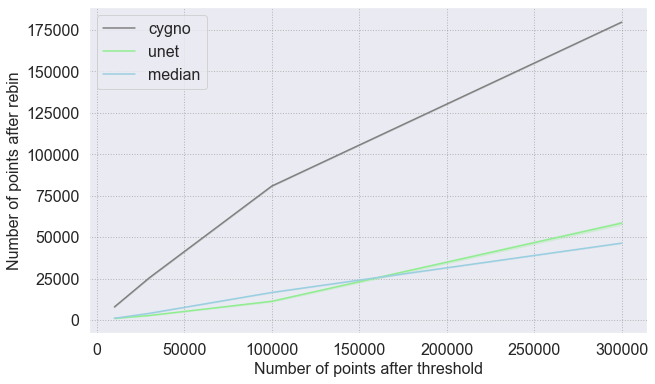
\includegraphics[width=0.7\textwidth]{image_files/rebinxinput.png}
\caption{Number of points after rebin}
\label{rebin_eval}
\end{figure}


Considering the scenario evaluated in the energy analysis, where it was possible to validate the equality for the distributions using a median filter and the algorithm used by the collaboration, the same process will be done for the analysis of the processing time, considering the both cases for 300000 points after threshold step.

In table \label{final_time}, its possible to notice a comparison between both proposes, processing all images. For median filter, the mean processing time for each image is 67.6, and it's possible to note a gain when compared to collaboration algorithm. This gain is close to 4.3 times faster.


\begin{tabular}{lrrrr}
\toprule
 Filter &  Total processing time (s) &  Clustering time (s) &  Number of images &  Time per image \\
\midrule
  cygno &              255081.7 &        207834.8 &               868 &      293.8 \\
 median &               58758.5 &         43249.6 &               868 &       67.6 \\
\bottomrule
\label{final_time}
\end{tabular}

\chapter{Conclusions}\label{chap:conclusions}


This work presents an initial proposal for constructing a simulation tool for modeling the ORANGE images for evaluation of image processing algorithms. The simulation tool was used to verify the importance of applying digital filters to the CYGNO images for improving their signal-to-noise ratio.



\section*{Acknowledgment}
The authors would like to thank the following Institutes/Universities for their valuable work: INFN-Roma I, Gran Sasso Science Institute L’Aquila, Dipartimento di Fisica della Sapienza Università di Roma, INFN-LNF, Museo Storico della Fisica e Centro Studi e Ricerche ”Enrico Fermi” and Post-Graduation Program in Electrical Engineering of UFJF.


\postextual 


%% Fizemos a op\c{c}\~ao por colocar as refer\^encias diretamente no arquivo ``.tex'' por ser mais simples para quem se inicia na escrita de trabalhos acad\^emicos.
%% Referencias. LISTAR EXATAMENTE AS CITADAS NO TRABALHO.

%No elemento REFER\^ENCIAS, todas ``as refer\^encias devem ser ... alinhadas \`a margem esquerda do texto ... (ABNT, 2018). 

\bibliographystyle{unsrt}
\bibliography{mybibliography.bib}

%% Apendices e Anexos nao devem ser subdivididos: A1, A2, etc.

%% Apendices

\begin{apendices}

\chapter{\apendseq T\'itulo} 
%%Digita-se o titulo do apendice mantendo-se, antes, o comando \apendseq, como indicado.

U-Net used architecture:

%\includegraphics{image_files/u-net.pdf}
\includepdf[pages=-]{image_files/u-net.pdf}

\end{apendices}

%% Anexos

\begin{anexos}

\chapter{\anexoseq T\'itulo} 
%%Digita-se o titulo do anexo mantendo-se, antes, o comando \anexoseq, como indicado.

Este elemento \'e opcional. Apresenta um texto ou documento \textbf{n\~ao} elaborado pelo autor com o objetivo de complementar ou comprovar sua 
argumenta\c{c}\~ao. 

  
\end{anexos}


%%% ---

\end{document}

%%%%EXEMPLO QUANDO SE TEM TODAS AS ILUSTRA\c{C}\~OES DO MESMO TIPO. POR EXEMPLO, ORGANOGRAMA.

%No meio do texto acima:
%1) coloque % antes de cada dos comandos \ilustvaria e \listilustvaria ;
%2) acrescente os dois comandos abaixo 

\tipoilust{Organograma} %Preencha com o tipo de sua ilustra\c{c}\~ao (somente caso todas sejam do mesmo tipo). Por exemplo, Organograma.
\renewcommand{\listfigurename}{\textbf{LISTA DE ORGANOGRAMAS}} %Troque ORGANOGRAMAS por outra palavra conforme o tipo de sua ilustra\c{c}\~ao, se for \'unico.

%3) retire % do in\'icio do comando 
\listoffigures* %Use este comando quando todas as ilustra\c{c}\~oes s\~ao do mesmo tipo e caso queira inserir a lista delas.

%Exemplo para se colocar a ilustrac\{c}\~ao neste caso, de tipo \'unico (por exemplo, Organograma) em todo o trabalho.

\begin{figure}[h]
\larguratexto{6cm}  %Mesma largura da ilustra\c{c}\~ao, dada em ``[width=6cm]'' abaixo
\begin{center}
\caption{Texto} %Substituir ``Texto'' pela informa\c{c}\~ao acima da ilustra\c{c}\~{a}o.
\includegraphics[width=6cm]{arquivo.jpg}
\fonte{Universidade Federal de Juiz de Fora (2012).} %%Indicar a fonte consultada (elemento obrigat\'orio, mesmo que seja produ\c{c}\~ao do pr\'oprio autor).
\end{center}
\end{figure}

